\documentclass[12pt,a5paper]{article}

% Russian language support
\usepackage[T2A]{fontenc}
\usepackage[utf8]{inputenc}
\usepackage[russian]{babel}

% Page layout
\usepackage[a5paper,margin=1.5cm]{geometry}
\usepackage{setspace}
\setstretch{1.06}

% Graphics and figures
\usepackage{graphicx}
\usepackage{float}

% Tables
\usepackage{longtable}
\usepackage{booktabs}
\usepackage{array}
\usepackage{tabularx}

% Mathematics
\usepackage{amsmath}
\usepackage{amssymb}
\usepackage{amsthm}
\newcommand{\Kcal}{\mathcal{K}}

% Hyperlinks
\usepackage{hyperref}
\hypersetup{
    colorlinks=true,
    linkcolor=black,
    citecolor=black,
    urlcolor=black
}

% Headers and footers
\usepackage{fancyhdr}
\pagestyle{fancy}
\fancyhf{}
\renewcommand{\headrulewidth}{0pt}
\fancyfoot[C]{\thepage}

% Section formatting
\usepackage{titlesec}
\titleformat{\section}{\centering\normalsize\bfseries}{\thesection}{1em}{}
\titleformat{\subsection}{\normalsize\bfseries}{\thesubsection}{1em}{}

% Reduce spacing
\titlespacing*{\section}{0pt}{8pt}{4pt}
\titlespacing*{\subsection}{0pt}{6pt}{3pt}

% Paragraph settings
\setlength{\parindent}{1.25cm}
\setlength{\parskip}{0pt}

\begin{document}
\sloppy

% Suppress page number on first page
\thispagestyle{empty}

% ============================================================
% TITLE PAGE
% ============================================================
\begin{center}
\textbf{Национальный исследовательский ядерный университет <<МИФИ>>}

\vspace{1cm}

\textit{На правах рукописи}

\vspace{2cm}

\textbf{Анаедевха Роджер Ник}

\vspace{1.5cm}

{\large \textbf{Состязательно-устойчивые модели и алгоритмы
повышения робастности и эффективности гибридных систем
обнаружения и предотвращения вторжений в распределённых
и нестационарных условиях}}

\vspace{1.5cm}

\textbf{2.3.1.\ Системный анализ, управление и обработка\\
информации, статистика\\
(технические науки)}

\vspace{2cm}

\textbf{АВТОРЕФЕРАТ}

\vspace{0.5cm}

диссертации на соискание ученой степени\\
кандидата технических наук

\vfill

Москва -- 2026
\end{center}

\newpage

% ============================================================
% PAGE 2 — Committee and defence details
% ============================================================
\thispagestyle{empty}
\enlargethispage{1cm}

{\footnotesize
\begin{center}
\textbf{Работа выполнена в федеральном государственном автономном\\
образовательном учреждении высшего образования\\
<<Национальный исследовательский ядерный университет <<МИФИ>>}
\end{center}

\vspace{0.2cm}

\noindent\begin{tabular}{@{}p{3cm}p{7.2cm}@{}}
\textbf{Научный руководитель:} & \textbf{Трофимов Александр Геннадьевич} \newline доктор физико-математических наук, профессор, профессор кафедры №~22 <<Кибернетика>> НИЯУ МИФИ \\
\end{tabular}

\vspace{0.2cm}

\noindent\textbf{Официальные оппоненты:}
\vspace{0.05cm}

\noindent\begin{tabular}{@{}p{3cm}p{7.2cm}@{}}
доктор технических наук, профессор, лауреат Премии Президента РФ в области образования, почётный работник науки и высоких технологий РФ \newline \textbf{Еремеев Александр Павлович} &
профессор кафедры прикладной математики и искусственного интеллекта ФГБОУ ВО <<Национальный исследовательский университет <<МЭИ>> \\[0.15cm]

доктор технических наук, профессор \newline \textbf{Калянов Георгий Николаевич} &
главный научный сотрудник Лаборатории инфраструктурных систем, ФГБУ ИПУ им.~В.\,А.~Трапезникова РАН \\
\end{tabular}

\vspace{0.2cm}

\noindent\begin{tabular}{@{}p{3cm}p{7.2cm}@{}}
\textbf{Ведущая организация:} & ФГБОУ ВО <<Тверской государственный технический университет>> \\
\end{tabular}

\vspace{0.2cm}

\noindent Защита состоится 30.06.2026 на заседании диссертационного совета~2.01 ФГАОУ ВО <<НИЯУ МИФИ>> (115409, г.~Москва, Каширское шоссе, 31)

\vspace{0.15cm}

\noindent С диссертацией можно ознакомиться в библиотеке и на сайте \url{https://ds.mephi.ru/} ФГАОУ ВО <<НИЯУ МИФИ>>

\vspace{0.15cm}

\noindent Автореферат разослан \underline{\hspace{2.5cm}} 2026

\vspace{0.3cm}

\noindent\begin{tabular}{@{}p{4.5cm}p{2cm}p{3.5cm}@{}}
Ученый секретарь диссертационного совета, кандидат физико-математических наук & & Климанов Сергей Геннадиевич \\
\end{tabular}
}

\newpage

% ============================================================
% MAIN CONTENT BEGINS
% ============================================================
\setcounter{page}{3}

\section*{ОБЩАЯ ХАРАКТЕРИСТИКА РАБОТЫ}
\addcontentsline{toc}{section}{Общая характеристика работы}

\subsection*{Актуальность темы исследования и степень её разработанности}

Гибридные системы обнаружения и предотвращения вторжений
(Hybrid Intrusion Detection and Prevention Systems, далее
Hybrid~IDPS) являются основным защитным контуром
информационно-телекоммуникационных систем критического
назначения~--- сетей сетевого трафика, защищаемых сегментов
центров обработки данных, инфраструктур беспилотных летательных
аппаратов, банковско-финансовых платформ, медицинских
информационных систем, промышленного интернета вещей и систем
управления критическими инфраструктурами. В отличие от
традиционных коммерческих продуктов (Snort, Suricata, Zeek,
Cisco~IPS, Palo~Alto, McAfee), которые опираются исключительно
на сигнатурный анализ и фиксированные правила, в настоящей
работе под Hybrid~IDPS понимается \emph{ИИ/МО-усиленный}
защитный контур, объединяющий три канонических типа
обнаружения~--- сигнатурный, поведенческий (аномалийный) и
анализ протоколов~--- в единую многоуровневую архитектуру с
обучаемыми компонентами и интегрированными средствами
реагирования.

Анализ инцидентов последних пяти лет в здравоохранении, финансовой
сфере, промышленном IoT, автономных системах и в самой
кибербезопасности показывает, что робастность развёрнутых
Hybrid~IDPS отстаёт от их детектирующей точности на
25--65~процентных пунктов: системы, демонстрирующие 95--98\%
обнаружения на эталонных данных, теряют 20--40\% точности под
адверсальными возмущениями входов, дрейфом распределения трафика,
византийскими нарушителями в распределённой архитектуре обучения
и при изменении профилей протоколов. К фундаментальным
неэффективностям современных Hybrid~IDPS относятся: запаздывание
сигнатур до 30--90~дней относительно появления новых угроз,
интенсивность ложных срабатываний $10^{-2}$--$10^{-1}$ на нормальный
поток и квадратичная по числу протоколов и сессий вычислительная
стоимость $\mathcal{O}(P\cdot S)$ протокольного анализа в режиме
реального времени.

В работе единая формализация Hybrid~IDPS выполнена в виде
кортежа $\mathcal{H} = (\mathcal{V}_t, \mathcal{E}_t, X_t, A_t,
f_\theta, g_\psi, \pi)$, где $\mathcal{V}_t$ и $\mathcal{E}_t$~---
изменяющиеся во времени множества сущностей и связей, $X_t$~---
матрица признаков, $A_t$~--- активные сигнатуры/правила,
$f_\theta$~--- обучаемый детектирующий модуль, $g_\psi$~---
модуль уверенности, $\pi$~--- политика реагирования. Шесть
сквозных свойств Hybrid~IDPS~--- состязательная устойчивость
(P1), робастность (P2), эффективность (P3), распределённость
(P4), человеческий фактор (P5) и нестационарность (P6)~---
формализованы как инвариантные условия и систематически
декомпозированы на семь подзадач, решаемых семью оригинальными
моделями и алгоритмами M1--M7. Графовые нейронные сети
используются в работе как одна из ветвей семейства обучаемых
моделей, применимых в Hybrid~IDPS, наряду со статистическими,
классическими ML, гибридными и теоретико-игровыми подходами.

Существенный вклад в области, образующие методологический
фундамент работы, внесли отечественные и зарубежные
исследователи: в обнаружение и предотвращение вторжений и
сетевую безопасность~--- А.\,А.~Бурлаков, А.\,С.~Марков,
В.\,В.~Сачков, M.~Roesch, V.~Paxson; в графовое глубокое
обучение~--- T.\,N.~Kipf, M.~Welling, P.~Veli\v{c}kovi\'{c},
W.\,L.~Hamilton; в нейронные ОДУ и пространства состояний~---
R.\,T.\,Q.~Chen, A.~Gu, T.~Dao; в адверсальное машинное
обучение~--- A.~Madry, N.~Carlini, D.~Wagner; в федеративное
обучение с приватностью~--- B.~McMahan, K.~Bonawitz,
H.~B.~McMahan; в теорию игр и сертификацию робастности~---
A.~Sinha, J.~Steinhardt, J.~Cohen. Однако ни один из
существующих подходов не обеспечивает одновременного выполнения
четырёх требований~--- робастности, точности, эффективности и
приватности~--- во всех трёх операционных условиях
Hybrid~IDPS: состязательной среде, нестационарности и
распределённой динамике обучения. Именно это противоречие между
многомерными требованиями и текущим состоянием алгоритмической
базы определяет актуальность настоящего исследования.

\subsection*{Объект и предмет исследования}

\textbf{Объектом исследования} являются \emph{гибридные системы
обнаружения и предотвращения вторжений} (Hybrid~IDPS),
функционирующие в состязательных, нестационарных и
распределённых средах и адаптируемые к различным предметным
областям~--- защите сетевого трафика, систем БПЛА, банковской
и финансовой инфраструктуры, систем хранения медицинских данных,
промышленного интернета вещей и систем управления критическими
инфраструктурами. Hybrid~IDPS объединяет сигнатурные,
поведенческие, протокольно-аналитические и обучаемые компоненты
в единый защитный контур с многоуровневой архитектурой и
интегрированными средствами реагирования.

\textbf{Предметом исследования} являются модели, алгоритмы и
специальное математическое обеспечение, повышающие робастность
и эффективность Hybrid~IDPS при сохранении состязательной
устойчивости, приватности распределённых данных и калиброванности
оценок неопределённости, включая аппарат непрерывно-временной
графовой динамики, селективных моделей пространств состояний,
федеративной оптимизации с дифференциальной приватностью,
оптимального транспорта, байесовского вывода и
теоретико-игровой сертификации.

\subsection*{Цель и задачи исследования}

\textbf{Целью} диссертационного исследования является повышение
робастности и эффективности гибридных систем обнаружения и
предотвращения вторжений (Hybrid~IDPS), функционирующих в
состязательных, нестационарных и распределённых условиях, за
счёт разработки единого математического описания Hybrid~IDPS и
семейства согласованных моделей и алгоритмов M1--M7, а также
доказательство применимости полученных результатов путём
инстанцирования в секторе защиты сетевого трафика
(NIDPS-сектор) и переноса в смежный сектор защиты бортовых
систем беспилотных летательных аппаратов.

\textbf{Задачи:}

\begin{enumerate}
\item Систематизировать существующие подходы к построению
Hybrid~IDPS в семи прикладных секторах, выявить пробелы и
сформулировать единые требования к разрабатываемым моделям и
алгоритмам.

\item Сформировать единое математическое описание Hybrid~IDPS
в виде кортежа $\mathcal{H} = (\mathcal{V}_t, \mathcal{E}_t,
X_t, A_t, f_\theta, g_\psi, \pi)$ и формализовать шесть
сквозных свойств P1--P6 в виде инвариантных условий, образующих
$3\times4$ матрицу <<условия$\times$требования>>.

\item Разработать семь моделей и алгоритмов M1--M7,
обеспечивающих покрытие двенадцати ячеек указанной матрицы:
непрерывно-временной графовой динамики CT-TGNN/SDE-TGNN~(M1);
федеративной оптимизации FedLLM-API с дифференциальной
приватностью~(M2); многоуровневых темпоральных эмбеддингов
TripleE-TGNN~(M3); селективной модели пространств состояний
MambaShield~(M4); калиброванного по неопределённости вывода
Stochastic Transformer/UC-HGP~(M5--M6); теоретико-игровой
сертификации FedGTD~(M7).

\item Инстанцировать Hybrid~IDPS для NIDPS-сектора, разработав
формальный конвейер преобразования сетевого трафика в графовые
структуры, унифицированную таксономию из~34 классов атак и
83-признаковый инженерный конвейер, согласованный с моделями
M1--M7.

\item Провести экспериментальную валидацию разработанных моделей
и алгоритмов на шести эталонных наборах данных общим объёмом
свыше 84,2~миллиона размеченных образцов и~84 уникальных
категорий атак с использованием унифицированной 23-метрической
системы оценки, включающей метрики точности, калибровки,
неопределённости, состязательной устойчивости, вычислительной
эффективности и приватности.

\item Реализовать единую программную платформу промышленного
уровня RobustIDPS.ai, объединяющую~17 нейросетевых моделей в~10
функциональных групп и~51 страницу пользовательского интерфейса
прогрессивного веб-приложения, и обеспечить её внедрение через
акты от четырёх организаций.

\item Подтвердить доменную независимость разработанных моделей
и алгоритмов путём их переноса в смежный сектор защиты
беспилотных летательных аппаратов с трёхъярусной архитектурой
<<борт~-- дронопорт~-- облако>>, а также экспериментальным
обоснованием кросс-доменного переноса в речевую обработку и
медицинские временные ряды.
\end{enumerate}

\subsection*{Методология и методы исследования}

В работе использовались методы системного анализа, теории
графов и спектральной теории графов, дифференциальных и
стохастических дифференциальных уравнений, функционального
анализа, теории оптимального транспорта, глубокого обучения,
байесовского вывода, теории информации, теории игр (равновесия
Штакельберга и Нэша), теории оптимизации, теории вероятностей,
математической статистики, теории дифференциальной
приватности, а также численных и вычислительных экспериментов
на эталонных корпусах данных. Используемая методология
обеспечивает единое формальное описание Hybrid~IDPS на уровне
кортежной модели и шести инвариантных свойств, что позволяет
доказательно увязать математические результаты M1--M7 с
прикладной задачей повышения робастности и эффективности.

\subsection*{Научная новизна работы}

\begin{enumerate}
\item \textit{Единое математическое описание Hybrid~IDPS.}
Впервые предложена кортежная формализация Hybrid~IDPS
$\mathcal{H} = (\mathcal{V}_t, \mathcal{E}_t, X_t, A_t, f_\theta,
g_\psi, \pi)$ и согласованная с ней система из шести
инвариантных свойств P1--P6, охватывающая состязательную
устойчивость, робастность, эффективность, распределённость,
человеческий фактор и нестационарность. На её основе построена
$3\times4$ матрица <<условия$\times$требования>>, упорядочивающая
семейство M1--M7 как покрытие всех двенадцати ячеек.

\item \textit{Непрерывно-временная темпоральная графовая
динамика для Hybrid~IDPS (CT-TGNN, SDE-TGNN).} Впервые в составе
Hybrid~IDPS использована модель, в которой представления узлов
эволюционируют по нейронным обыкновенным дифференциальным
уравнениям на изменяющихся во времени графах, а сертифицированные
границы робастности выводятся из неравенства Гронуолла. Стохастическое
расширение SDE-TGNN заменяет детерминированную динамику
уравнениями Ито и аналитически распространяет первые два
момента через уравнение Фоккера--Планка. Достигнуты F1
99,0\%, ECE 0,042, сертифицированная робастность 76,2\% при
радиусе $R{=}0{,}25$ и кросс-доменный перенос 90,5\% F1 без
дообучения.

\item \textit{Византийско-устойчивая федеративная оптимизация
для Hybrid~IDPS (FedLLM-API).} Разработан оригинальный
федеративный оптимизатор, совместно обеспечивающий покоординатное
усечённое среднее, $(\varepsilon{=}0{,}85,\delta{=}10^{-5})$
дифференциальную приватность и выравнивание распределений
гетерогенных клиентов через расстояние Вассерштейна. Доказана
сходимость со скоростью $\mathcal{O}(1/\sqrt{T})$ при
30\%~повреждённых участников; при 40\%~византийских участниках
обеспечена точность 87,1\% против 61,4\% у FedAvg. Интеграция
LLM обеспечивает 87,6\% F1 при детектировании новых классов
атак.

\item \textit{Многоуровневые темпоральные графовые эмбеддинги
для Hybrid~IDPS (TripleE-TGNN).} Разработана архитектура
тройных эмбеддингов на уровнях сервисов, трассировок и узлов
с двойным темпорально-пространственным вниманием и эластичной
консолидацией весов, противодействующей катастрофическому
забыванию. Достигнута точность 96,8\% при снижении
вычислительной стоимости на 40\% и сохранении 94,7\% точности
без дообучения при непрерывной эволюции топологии.

\item \textit{Селективные модели пространств состояний для
Hybrid~IDPS (MambaShield).} Разработана архитектура с
БПФ-свёртками, снижающая сложность вывода с $\mathcal{O}(L^2)$
до $\mathcal{O}(L\log L)$ и интегрирующая прогрессивную
дистилляцию состязательной робастности. При 25\% отравлении
обучающих данных достигнута точность 91,4\% против 73,8\% у
незащищённой модели; PAC-байесовские сертификаты обобщения
подтверждены с погрешностью 2,7\%; латентность вывода
0,5~мс/поток.

\item \textit{Калиброванный по неопределённости вывод для
Hybrid~IDPS (Stochastic Transformer, UC-HGP).} Впервые в составе
Hybrid~IDPS разработана интеграция вариационного байесовского
внимания с иерархическими гауссовскими процессами, обеспечивающая
эпистемически-алеаторную декомпозицию неопределённости с ECE
0,078 (снижение на 59\% относительно детерминированного
внимания) и сокращение нагрузки аналитика на 43\% за счёт
приоритизации по уровню неопределённости.

\item \textit{Теоретико-игровая сертификация Hybrid~IDPS
(FedGTD).} Построен оригинальный механизм сертификации
робастности через равновесия Штакельберга с алгоритмом
мультипликативных весов, для которого доказана граница
сожаления $R(T)\le 2\sqrt{T\log|\mathcal{C}|}$. Регуляризация
согласованности связывает все семь моделей с доказанной
сходимостью. Точность 94,7\% против адаптивных противников
против 87,6\% у нестратегических подходов.

\item \textit{Доменно-специфическая фундаментальная модель
(CyberSecLLM).} Разработана архитектура с ODE-дополненными
селективными блоками пространств состояний, достигшая средней
zero-shot точности 89,1\% на 11-задачном эталоне CyberSecBench~---
улучшение на 20,5~пункта относительно GPT-4 при обработке
миллион-токенных последовательностей графовых событий за
2,3~секунды.
\end{enumerate}

\subsection*{Теоретическая значимость}

Теоретическая значимость состоит в построении единого
математического описания Hybrid~IDPS как объекта исследования
и интегрированной системы доказательств, связывающей пять
формальных дисциплин: нейронных обыкновенных и стохастических
дифференциальных уравнений (CT-/SDE-TGNN, MambaShield),
оптимального транспорта и теории дифференциальной приватности
(FedLLM-API), селективных моделей пространств состояний и
БПФ-свёрток (MambaShield), вариационного байесовского вывода
и иерархических гауссовских процессов (Stochastic Transformer,
UC-HGP) и теории игр со стохастическим обучением без сожаления
(FedGTD). Совместное применение этих аппаратов даёт формальные
гарантии сходимости, устойчивости, приватности и обобщения,
верифицируемые как теоретически, так и эмпирически, и
впервые увязывает их в единый научно-методический каркас
повышения робастности и эффективности Hybrid~IDPS.

\subsection*{Практическая значимость}

Практическая значимость определяется разработкой моделей,
алгоритмов и специального программного обеспечения для
построения Hybrid~IDPS, применимых в секторе защиты сетевого
трафика, бортовых систем БПЛА, банковской и финансовой
инфраструктуры, медицинских информационных систем, промышленного
интернета вещей и других. Разработанная система обеспечивает:

\begin{itemize}
\item высокую точность обнаружения (94,7\% на CIC-IoT-2023)
с одновременной состязательной устойчивостью;
\item сохранение приватности данных в распределённых
архитектурах за счёт федеративного обучения с
$(\varepsilon{=}0{,}85,\delta{=}10^{-5})$ дифференциальной
приватностью;
\item работу в режиме реального времени: 8,7~млн событий/с при
латентности 47~мс и инференсе 0,5~мс/поток для MambaShield;
\item совместимость с эволюционирующими протоколами, в том
числе с пост-квантовыми криптографическими стандартами
(модуль Multi-Agent PQC-IDS, 96,2\%);
\item кросс-доменную переносимость: 90,5\% F1 без дообучения,
подтверждённую на речевых (LibriSpeech) и медицинских
(MIMIC-III/eICU) корпусах.
\end{itemize}

Практическая значимость подтверждена выпуском
программной платформы RobustIDPS.ai (DOI:~10.5281/zenodo.19129512),
интегрирующей \textbf{17~нейросетевых моделей} в
\textbf{10~функциональных групп} и \textbf{51~страницу}
прогрессивного веб-приложения, четырёхуровневую систему защиты
LLM (94,5\% обнаружения по 517 сценариям атак с четырьмя
коммерческими бэкендами), а также модулем Multi-Agent PQC-IDS,
и подтверждена актами внедрения от четырёх организаций:
Госкорпорации <<Росатом>> (95,7\%), ООО <<Позитив Текнолоджиз>>
(федеративное обучение для коммерческих IDPS), Google~Cloud
Platform (96,8\% точности, снижение затрат на 40\%) и
Suricata Open~Source~IDPS (адаптивный плагин с адаптацией к
дрейфу концепций).

\subsection*{Достоверность научных результатов}

Достоверность обеспечивается: строгой математической
формализацией Hybrid~IDPS как кортежной модели и шести свойств
P1--P6 с доказательствами сходимости, устойчивости, приватности
и сложности; экспериментальной валидацией на шести открытых
наборах данных общим объёмом 84,2~млн размеченных образцов и
84~уникальных категорий атак; сравнительным анализом с
современными базовыми и состояния-искусства методами с
превосходством на 2,9--5,6~процентных пунктов; абляционными
исследованиями, подтверждающими измеримый вклад каждого
компонента M1--M7; экспериментами под шестью семействами
состязательных атак; кросс-доменным переносом; представлением
на международных конференциях, публикациями в ведущих
рецензируемых журналах (Scopus/Web of Science) и актами
внедрения от четырёх организаций.

\subsection*{Апробация результатов исследования}

Основные положения и результаты были представлены и обсуждены
на следующих международных и российских научных конференциях:

\begin{enumerate}
\item 2024 Conference of Young Researchers in Electrical and
Electronic Engineering (ElCon-2024), Saint Petersburg, Russia, IEEE;
\item 2025 Conference of Young Researchers in Electrical and
Electronic Engineering (ElCon-2025), ETU-LETI, Saint Petersburg,
Russia, IEEE;
\item International Conference ``Advances in Neural Computation,
Machine Learning, and Cognitive Research~IX''
(NEUROINFORMATICS-2025), Springer;
\item Третья Всероссийская научно-техническая конференция
<<Кибернетика и информационная безопасность>> (КИБ-2025),
НИЯУ МИФИ, Москва;
\item 2026 IEEE 27th International Conference of Young
Professionals in Electron Devices and Materials (EDM-2026),
Altai Republic, Russia;
\item 11th IEEE Electronics System-Integration Technology
Conference (IEEE ESTC 2026), Helsinki, Finland;
\item IEEE Research and Technologies for Society and Industry
(RTSI) 2026 Conference, Espoo, Finland;
\item NeurIPS 2026: The 40th Annual Conference on Neural
Information Processing Systems, Sydney, Australia.
\end{enumerate}

\subsection*{Публикации}

Основные результаты опубликованы в 18~научных работах, включая:
5~статей в рецензируемых журналах, индексируемых в Scopus и Web
of Science (Neurocomputing, Expert Systems with Applications,
Complex and Intelligent Systems, Optical Memory and Neural
Networks, IJASRE); 4~статьи в трудах международных конференций
(Scopus, IEEE~Xplore); 2~статьи, принятые к публикации
(Knowledge and Information Systems, Complex and Intelligent
Systems); 7~статей на рецензировании в ведущих журналах
IEEE~Transactions и других изданиях.

\subsection*{Основные научные результаты, выносимые на защиту}

Результаты, выносимые на защиту, перечислены в порядке,
отражающем их логические зависимости в рамках единого
математического описания Hybrid~IDPS; каждый последующий
результат опирается на гарантии, установленные предыдущими.

\begin{enumerate}
\item Единое математическое описание Hybrid~IDPS в виде
кортежа $\mathcal{H} = (\mathcal{V}_t, \mathcal{E}_t, X_t, A_t,
f_\theta, g_\psi, \pi)$ и системы шести инвариантных свойств
P1--P6, образующих $3\times4$ матрицу
<<условия$\times$требования>>, на основе которой выстраивается
семейство M1--M7.

\item Модели CT-TGNN и SDE-TGNN сертифицированной
непрерывно-временной графовой динамики, в которых нейронные
ОДУ/СДУ управляют эволюцией представлений узлов и рёбер на
изменяющихся во времени топологиях, а сертифицированные границы
робастности выводятся из неравенства Гронуолла и аналитического
распространения моментов через уравнение Фоккера--Планка.

\item Алгоритм FedLLM-API византийско-устойчивой федеративной
оптимизации с доказанной сходимостью $\mathcal{O}(1/\sqrt{T})$,
формальной дифференциальной приватностью
$(\varepsilon{=}0{,}85,\delta{=}10^{-5})$ и выравниванием
распределений на основе оптимального транспорта, обеспечивающий
совместное обучение участников Hybrid~IDPS в условиях
византийских нарушителей и контролируемого бюджета приватности.

\item Архитектура TripleE-TGNN многоуровневых темпоральных
графовых эмбеддингов и архитектура MambaShield селективной
модели пространств состояний со сложностью $\mathcal{O}(L\log L)$,
совместно обеспечивающие выполнение требований эффективности
и устойчивости к отравлению Hybrid~IDPS при непрерывной
эволюции топологии.

\item Модели Stochastic Transformer и UC-HGP калиброванного
по неопределённости вывода с эпистемически-алеаторной
декомпозицией и сублинейной границей сожаления для адаптации
Hybrid~IDPS к нестационарным распределениям с поддержкой
человеческого фактора (триаж и приоритизация).

\item Теоретико-игровая система сертификации FedGTD,
интегрирующая гарантии результатов~(2)--(5) в единую методологию
оценки через равновесия Штакельберга и регуляризацию
согласованности, и доменно-специфическая фундаментальная
модель CyberSecLLM.

\item Программная реализация результатов в виде платформы
RobustIDPS.ai с 17~нейросетевыми моделями в 10~функциональных
группах и 51~странице веб-приложения, валидированная на шести
эталонных наборах данных (84,2~млн образцов, 84~категории атак)
и подтверждённая четырьмя актами внедрения, а также
инстанцирование того же каркаса в смежном секторе защиты
бортовых систем БПЛА.
\end{enumerate}

\subsection*{Соответствие паспорту научной специальности}

Диссертация соответствует специальности 2.3.1 <<Системный
анализ, управление и обработка информации, статистика>>:

\noindent П.4 <<Разработка методов и алгоритмов решения задач
системного анализа, оптимизации, управления, принятия решений,
обработки информации и искусственного интеллекта.>> ---
соответствие подтверждается разработкой семи оригинальных
моделей и алгоритмов M1--M7 для задач обнаружения и
предотвращения вторжений и обработки графовых потоков сетевого
трафика в Hybrid~IDPS.

\noindent П.5 <<Разработка специального математического и
алгоритмического обеспечения систем анализа, оптимизации,
управления, принятия решений, обработки информации и
искусственного интеллекта.>> --- соответствие подтверждается
формализацией Hybrid~IDPS в виде кортежной модели и шести
инвариантных свойств P1--P6, а также реализацией единой
программной платформы RobustIDPS.ai с 17~интегрированными
нейросетевыми моделями.

\subsection*{Структура и объём диссертации}

Диссертация состоит из введения, шести глав, заключения,
библиографического списка и трёх приложений. Основной текст
составляет 230~страниц. Библиографический список содержит
204~наименования. Глава~1 содержит системный анализ Hybrid~IDPS
в семи прикладных секторах и формулирует пробелы. Глава~2 даёт
единое математическое описание Hybrid~IDPS и семейство моделей
M1--M7. Глава~3 инстанцирует это описание в NIDPS-секторе.
Глава~4 представляет экспериментальную валидацию. Глава~5
описывает программную платформу RobustIDPS.ai. Глава~6
демонстрирует перенос разработанного каркаса в сектор защиты
бортовых систем БПЛА.

\section*{ОСНОВНОЕ СОДЕРЖАНИЕ РАБОТЫ}
\addcontentsline{toc}{section}{Основное содержание работы}

\textbf{Во введении} обоснована актуальность темы, определены
объект (Hybrid~IDPS) и предмет (модели и алгоритмы повышения
робастности и эффективности), сформулирована цель и семь задач
исследования, изложены научная новизна, теоретическая и
практическая значимость, основные положения, выносимые на
защиту, апробация результатов и структура диссертации.

\textbf{Глава~1} проводит системный анализ Hybrid~IDPS в семи
прикладных секторах (защита сетевого трафика, банковско-финансовый
сектор, здравоохранение, промышленный IoT, бортовые системы
БПЛА, облачные и микросервисные среды, государственное
управление и критические инфраструктуры) и фиксирует пробелы,
которые невозможно закрыть в рамках одной модели. Глава
описывает три канонических типа обнаружения (сигнатурный,
поведенческий, протокольно-аналитический) и выявляет их
ограничения, а также формулирует требования к разрабатываемым
моделям и алгоритмам. На рисунке~\ref{fig:nidps_overview}
показан исполнительный обзор контура NIDPS как одной из основных
инстанций Hybrid~IDPS.

% ============================================================
% FIGURE 1: NIDPS Executive Overview
% ============================================================
\begin{figure}[H]
\centering
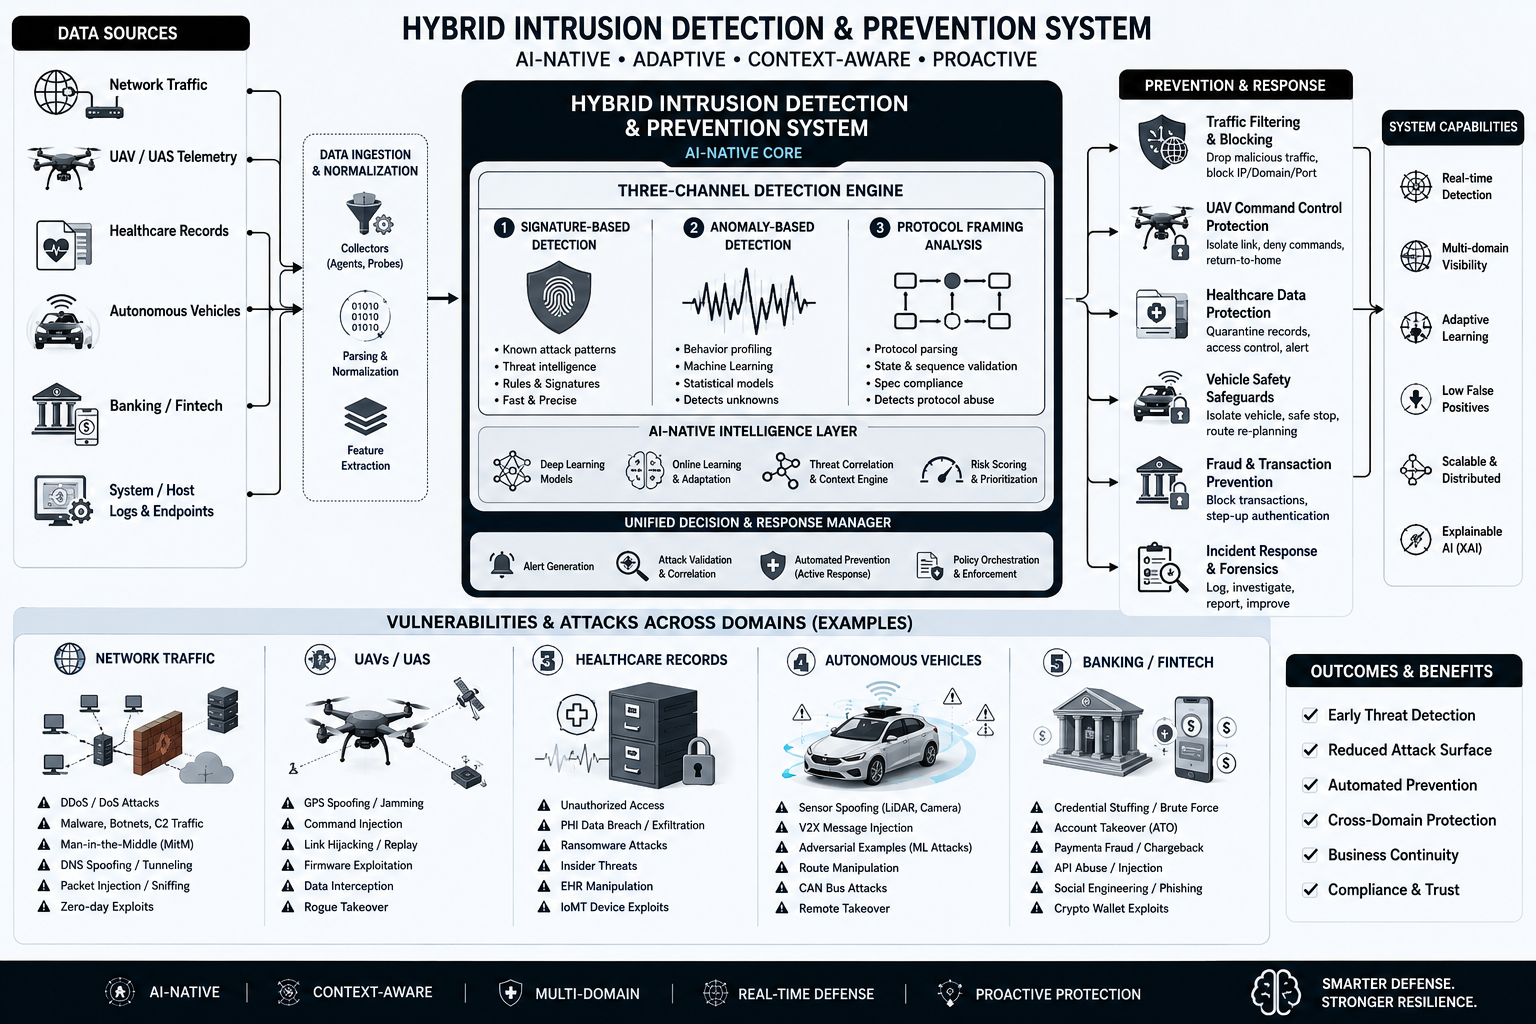
\includegraphics[width=0.92\textwidth]{figures/fig_nidps_v1.png}
\caption{Исполнительный обзор сетевой инстанции Hybrid~IDPS
(NIDPS): обучаемый контур поверх сигнатурных и поведенческих
детекторов}
\label{fig:nidps_overview}
\end{figure}

\textbf{Глава~2} формализует Hybrid~IDPS как кортеж
$\mathcal{H} = (\mathcal{V}_t, \mathcal{E}_t, X_t, A_t,
f_\theta, g_\psi, \pi)$ и шесть инвариантных свойств
P1--P6 (рисунок~\ref{fig:main_arch}). На этой основе строится
семейство M1--M7, образующее покрытие $3\times4$ матрицы
<<условия$\times$требования>>.

% ============================================================
% FIGURE 2: Research Framework Matrix
% ============================================================
\begin{figure}[H]
\centering
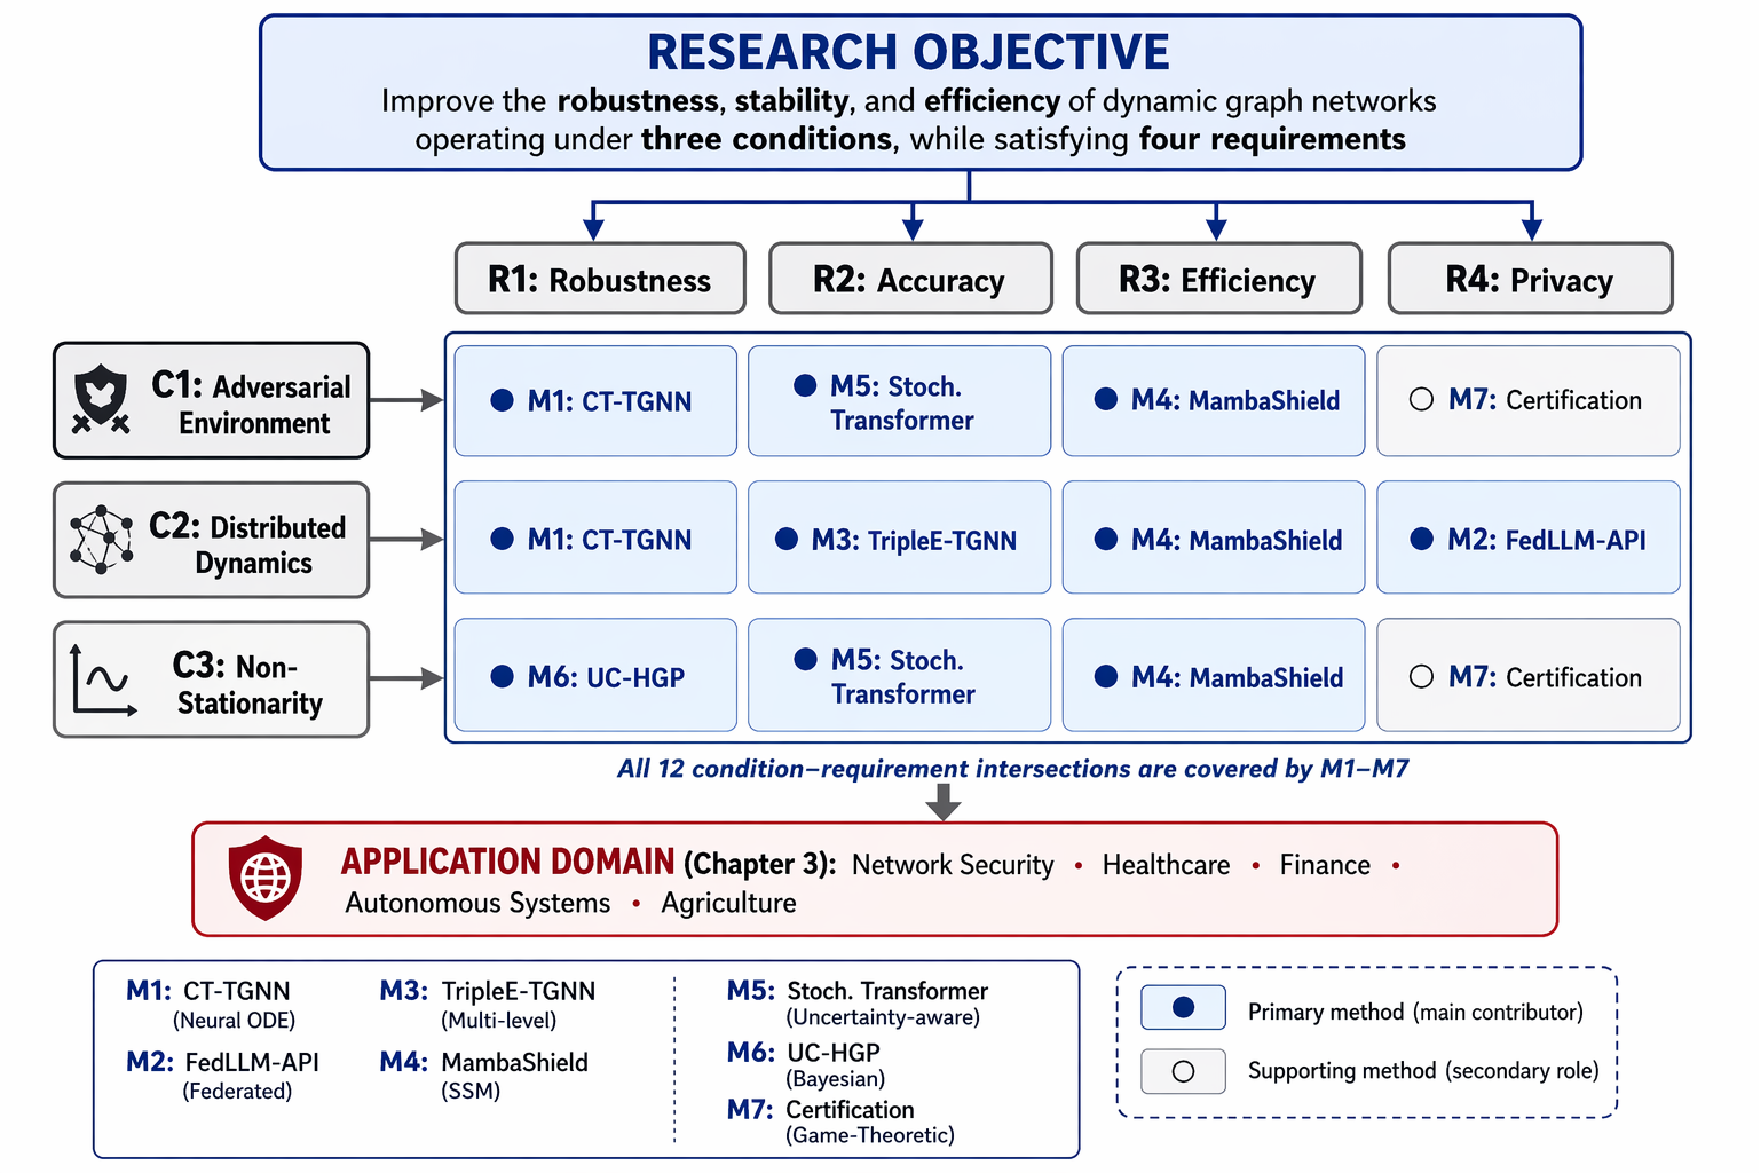
\includegraphics[width=0.96\textwidth]{figures/Main_arch_v1.pdf}
\vspace{-0.5cm}
\caption{Архитектурная основа единого математического описания
Hybrid~IDPS: семейство M1--M7 покрывает все двенадцать ячеек
матрицы <<условия$\times$требования>>}
\label{fig:main_arch}
\end{figure}

\textit{Модель M1: CT-TGNN/SDE-TGNN --- непрерывно-временная
графовая динамика для Hybrid~IDPS.} Эволюция представлений
узлов задаётся параметризованным дифференциальным оператором
на изменяющейся во времени топологии:
\begin{equation}
\frac{dh_v(t)}{dt} = f_\theta\bigl(h_v(t), A(t), X(t), t\bigr).
\end{equation}
Сопряжённый метод чувствительности обеспечивает обучение с
$\mathcal{O}(1)$ по памяти; темпоральная адаптивная пакетная
нормализация согласует непрерывную динамику со слоями нормализации.

\textbf{Теорема~1 (Сходимость).} При константе Липшица $L_f$
и скорости обучения $\eta < 2/L_f$ обучение сходится со
скоростью $\mathcal{O}(1/\sqrt{T})$.

\textbf{Теорема~2 (Сертифицированная робастность).} Для входных
возмущений $\|\delta X\|\le\varepsilon$ выходная чувствительность
ограничена по неравенству Гронуолла
$\|\delta h(T)\|\le\varepsilon L_g T\exp(L_g T)$.

% ============================================================
% FIGURE: CT-TGNN
% ============================================================
\begin{figure}[H]
\centering
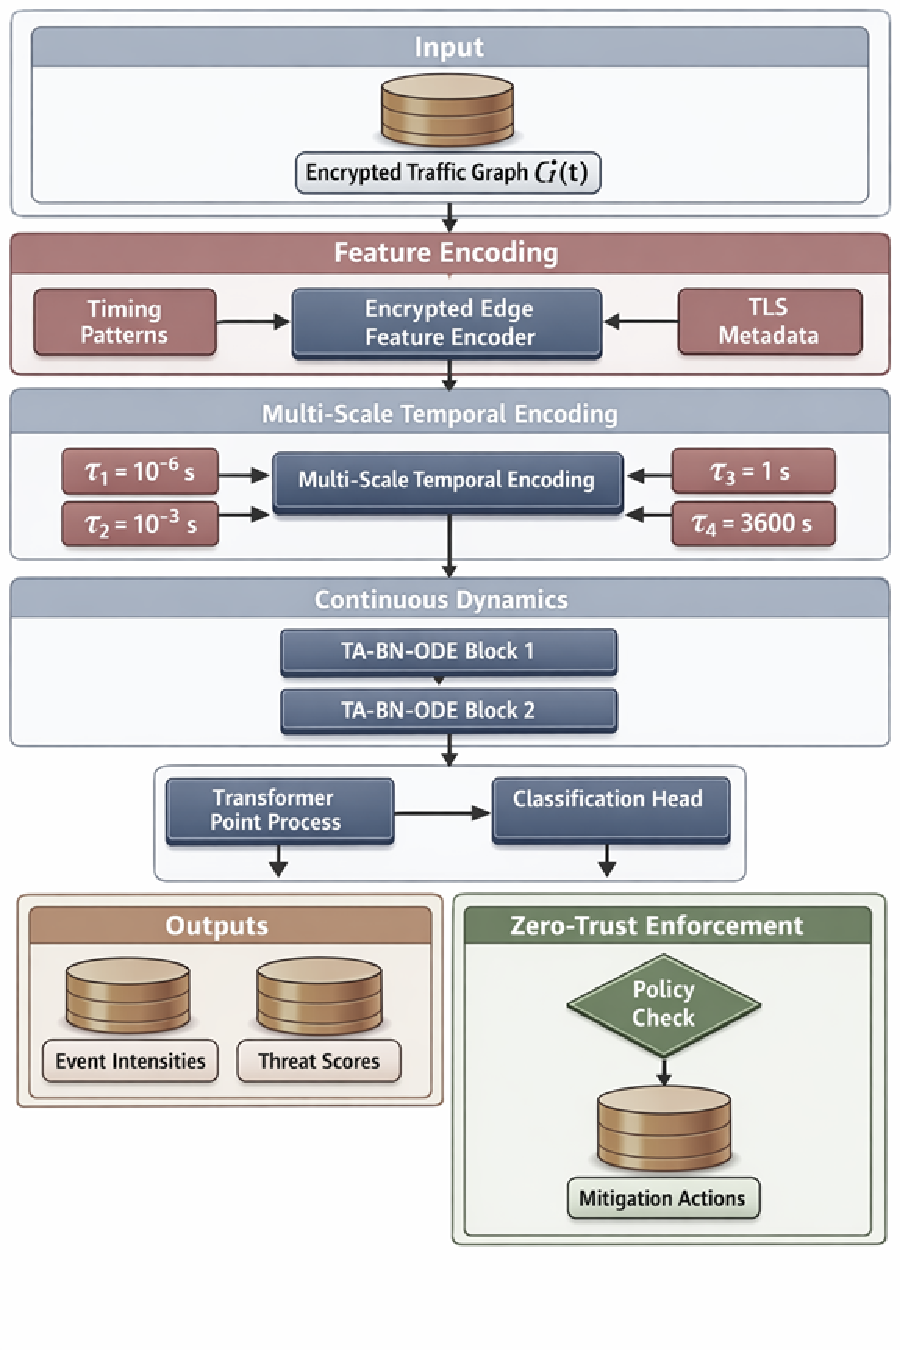
\includegraphics[width=0.70\textwidth]{figures/fig_CT-TGNN_architecture.pdf}
\vspace{-0.5cm}
\caption{Архитектура CT-TGNN: непрерывно-временная графовая
динамика как обучаемый компонент Hybrid~IDPS}
\label{fig:CT-TGNN}
\end{figure}

Стохастическое расширение SDE-TGNN заменяет детерминированную
динамику стохастическими дифференциальными уравнениями Ито и
аналитически распространяет среднее и ковариацию через уравнение
Фоккера--Планка, давая сертифицированный радиус через
сглаживание классификатора (рисунок~\ref{fig:SDE_TGNN}). Достигнуты
F1 99,0\%, ECE 0,042, сертифицированная состязательная
устойчивость 76,2\% при $R{=}0{,}25$ и кросс-доменный перенос
90,5\%~F1.

\begin{figure}[H]
\centering
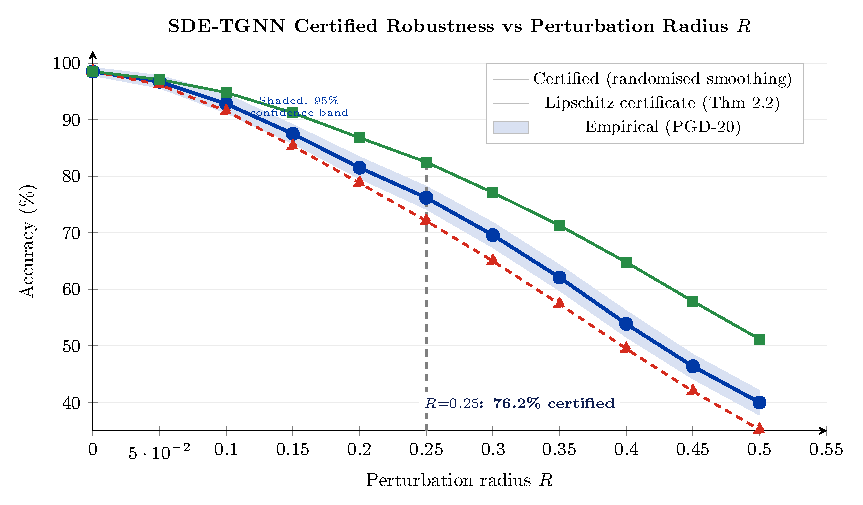
\includegraphics[width=0.80\textwidth]{figures/fig_sde_tgnn_robustness_vs_radius.pdf}
\vspace{-0.3cm}
\caption{SDE-TGNN: сертифицированная точность как функция
радиуса возмущения}
\label{fig:SDE_TGNN}
\end{figure}

\textit{Модель M2: FedLLM-API --- федеративная оптимизация
Hybrid~IDPS с приватностью.} Покоординатная агрегация с
калиброванным гауссовским шумом и выравнивание распределений
по Вассерштейну:
\begin{equation}
\theta_{t+1}=\text{TrimMean}\!\left(\{\theta_i^t\}_{i=1}^{N}\right)
+\mathcal{N}(0,\sigma^2 I),\quad
W_2(\mu_i,\mu_j)=\!\!\inf_{\pi\in\Pi(\mu_i,\mu_j)}\!\!
\sqrt{\int\!\!\|x-y\|^2 d\pi}.
\end{equation}

\textbf{Теорема~3 (Сходимость при повреждениях).} Алгоритм
сходится со скоростью $\mathcal{O}(1/\sqrt{T})$ даже при 30\%
повреждённых участников при сохранении
$(\varepsilon{=}0{,}85,\delta{=}10^{-5})$-приватности.

\begin{figure}[H]
\centering
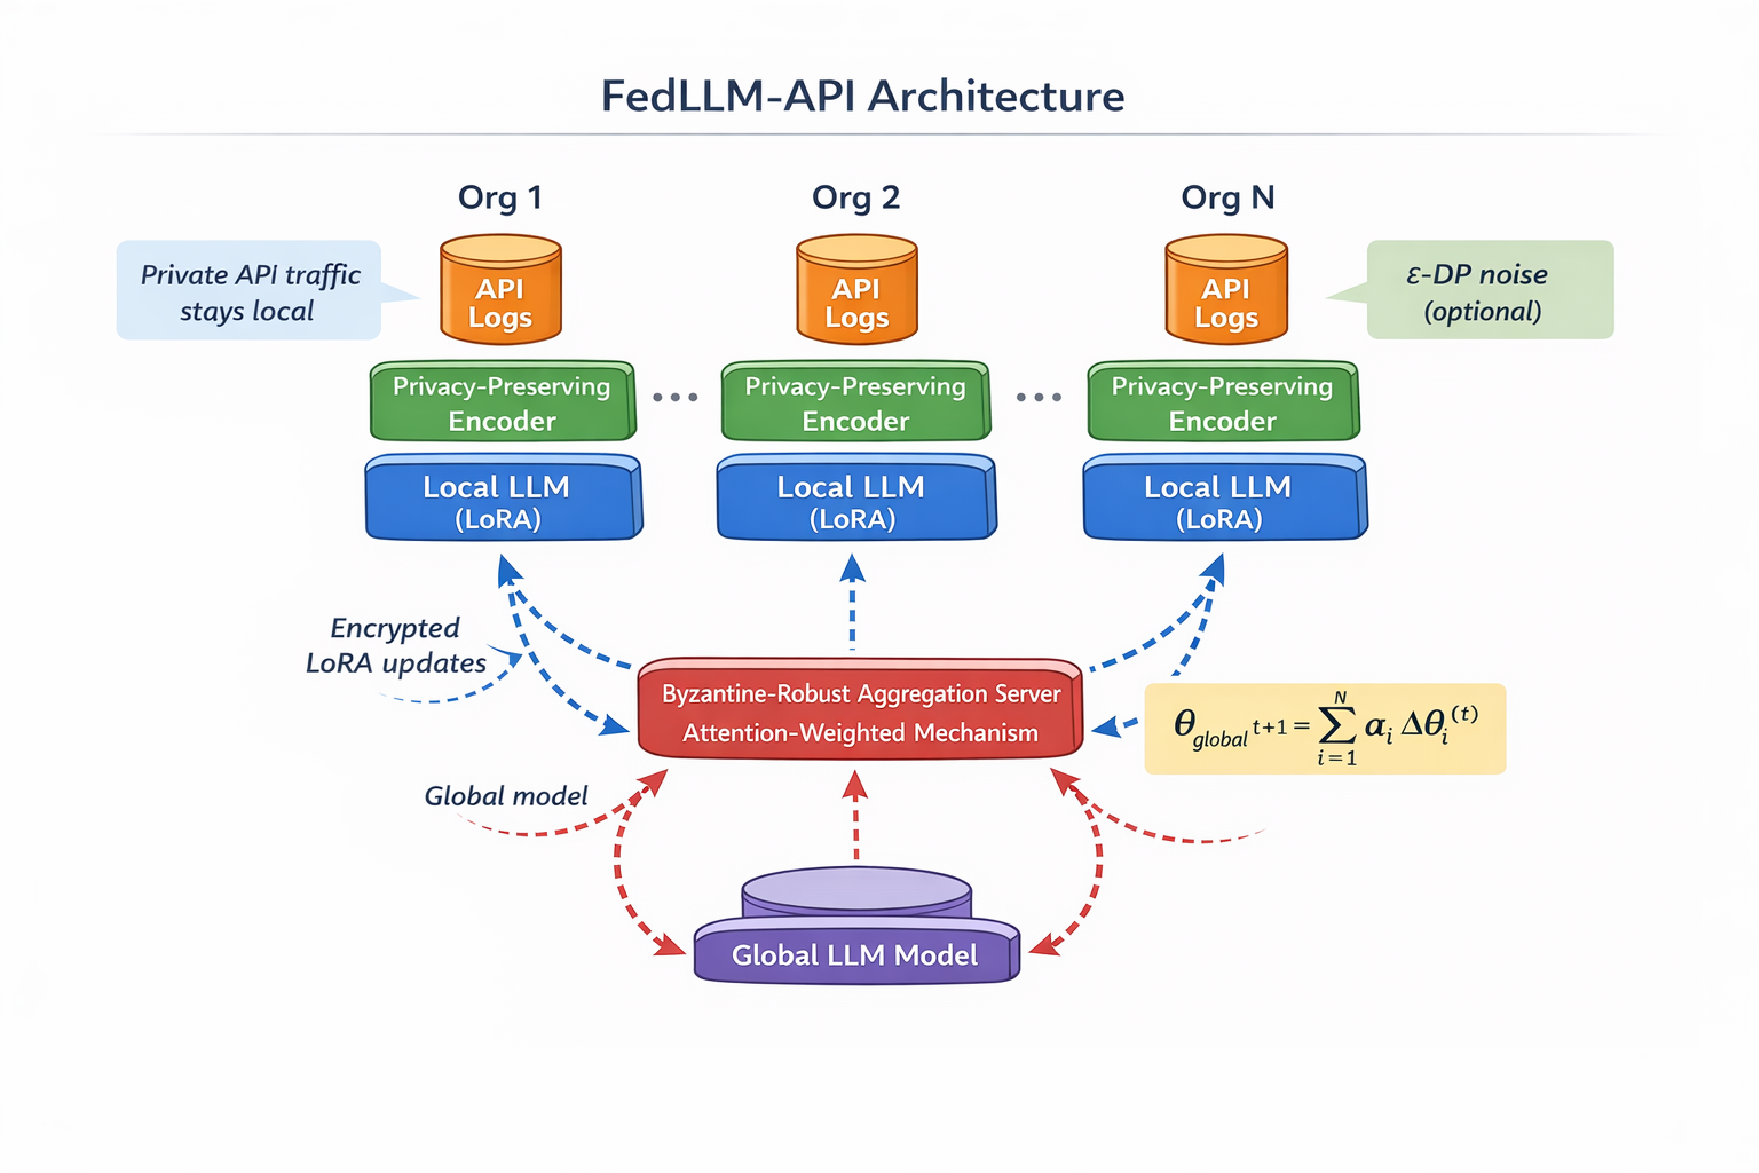
\includegraphics[width=0.80\textwidth]{figures/fig_fedllm_api_architecture.pdf}
\vspace{-0.3cm}
\caption{Архитектура FedLLM-API: византийско-устойчивая
федеративная оптимизация Hybrid~IDPS с дифференциальной
приватностью}
\label{fig:FedLLM}
\end{figure}

Интеграция LLM даёт 87,6\% F1 при детектировании новых
аномальных категорий в режиме zero-shot; при 40\% византийских
участников точность 87,1\% против 61,4\% у FedAvg.

\textit{Модель M3: TripleE-TGNN --- многоуровневые темпоральные
графовые эмбеддинги.} Двойное темпорально-пространственное
внимание и эластичная консолидация весов:
\begin{equation}
\alpha_{uv}^{(t)}=\frac{\exp(e_{uv}^{(t)})}{\sum_{w}\exp(e_{vw}^{(t)})},\qquad
\mathcal{L}_{\text{EWC}}=\mathcal{L}_{\text{task}}
+\frac{\lambda}{2}\sum_i F_i(\theta_i-\theta_i^*)^2.
\end{equation}

\begin{figure}[H]
\centering
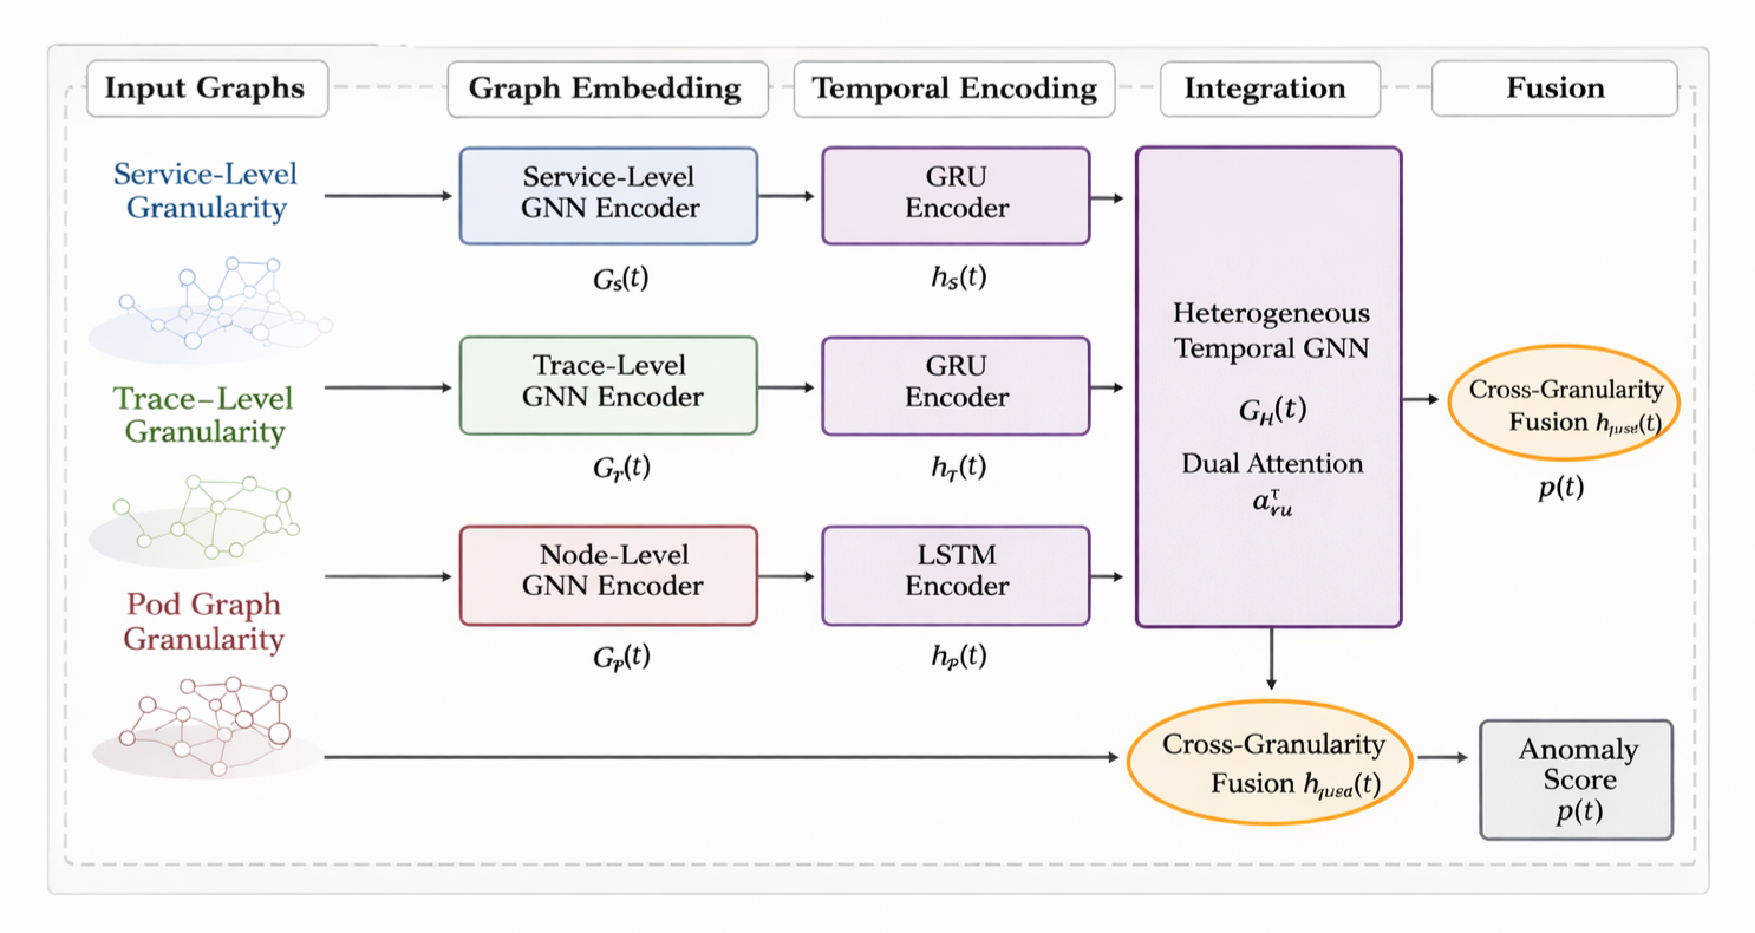
\includegraphics[width=0.95\textwidth]{figures/fig_triplee_tgnn_architecture.pdf}
\vspace{-0.4cm}
\caption{Архитектура TripleE-TGNN: представления на уровнях
сервисов, трассировок и узлов с эластичной консолидацией
весов}
\label{fig:TripleE_TGNN}
\end{figure}

Достигнута точность 96,8\% и снижение вычислительных затрат
на 40\% за счёт структурированной разреженности.

\textit{Модель M4: MambaShield --- селективная модель
пространств состояний с защитой от отравления.} Дискретная
формулировка пространства состояний и БПФ-свёртки:
\begin{equation}
h_{t+1}=\bar{A}h_t+\bar{B}x_t,\quad
y_t=Ch_t+Dx_t,\qquad
\mathcal{L}_{\text{distill}}=\text{KL}\!\left(p_{\text{st}}
\Big\|\frac{1}{K}\sum_k p_{\text{tch}_k}\right).
\end{equation}

\textbf{Теорема~4 (PAC-байесовское обобщение).}
\begin{equation}
R(\theta)\le\hat{R}(\theta)
+\sqrt{\frac{\text{KL}(\rho\|\pi)+\ln(2N/\delta)}{2N}}.
\end{equation}

\begin{figure}[H]
\centering
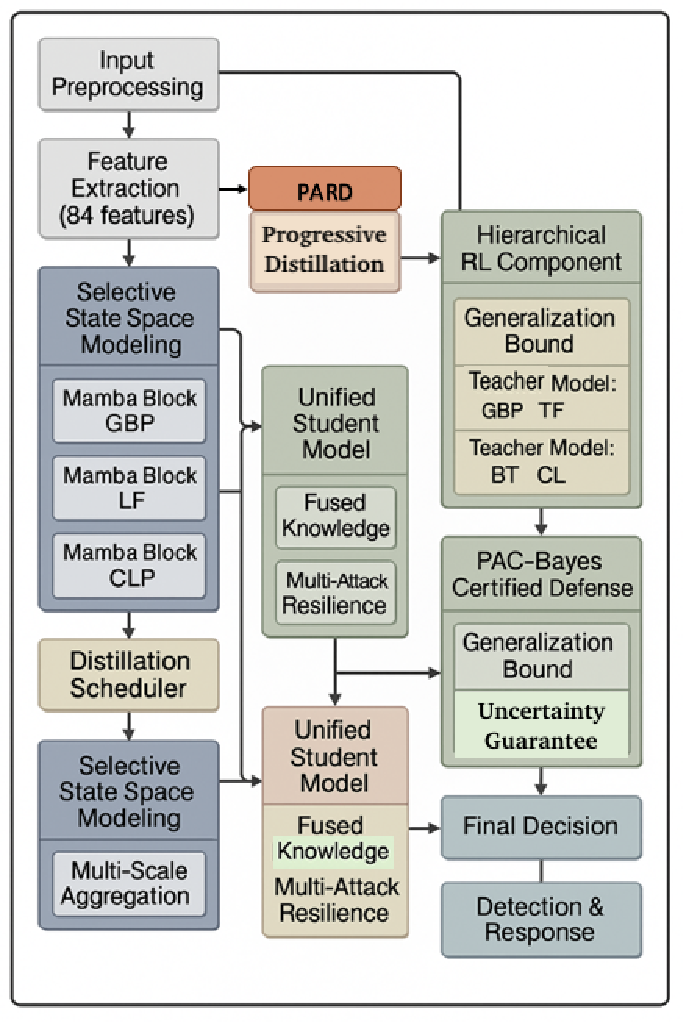
\includegraphics[width=0.65\textwidth]{figures/fig_mambashield_architecture.pdf}
\vspace{-0.3cm}
\caption{Архитектура MambaShield: $\mathcal{O}(L\log L)$
БПФ-свёртки с прогрессивной дистилляцией состязательной
робастности}
\label{fig:mambashield}
\end{figure}

При 25\% отравлении достигнута точность 91,4\% против 73,8\% у
незащищённой модели; латентность вывода 0,5~мс/поток.

\textit{Модели M5/M6: Stochastic Transformer и UC-HGP ---
калиброванный по неопределённости вывод.} Вариационное
байесовское внимание и иерархический гауссовский процесс:
\begin{equation}
q_\phi(\alpha)=\mathcal{N}(\mu_\phi,\sigma_\phi^2),\qquad
\mathcal{L}=\mathbb{E}_{q_\phi}[\log p(y|x,\alpha)]
-\text{KL}(q_\phi\|p),\qquad
f(x)\sim\mathcal{GP}(m(x),k(x,x')).
\end{equation}

\begin{figure}[H]
\centering
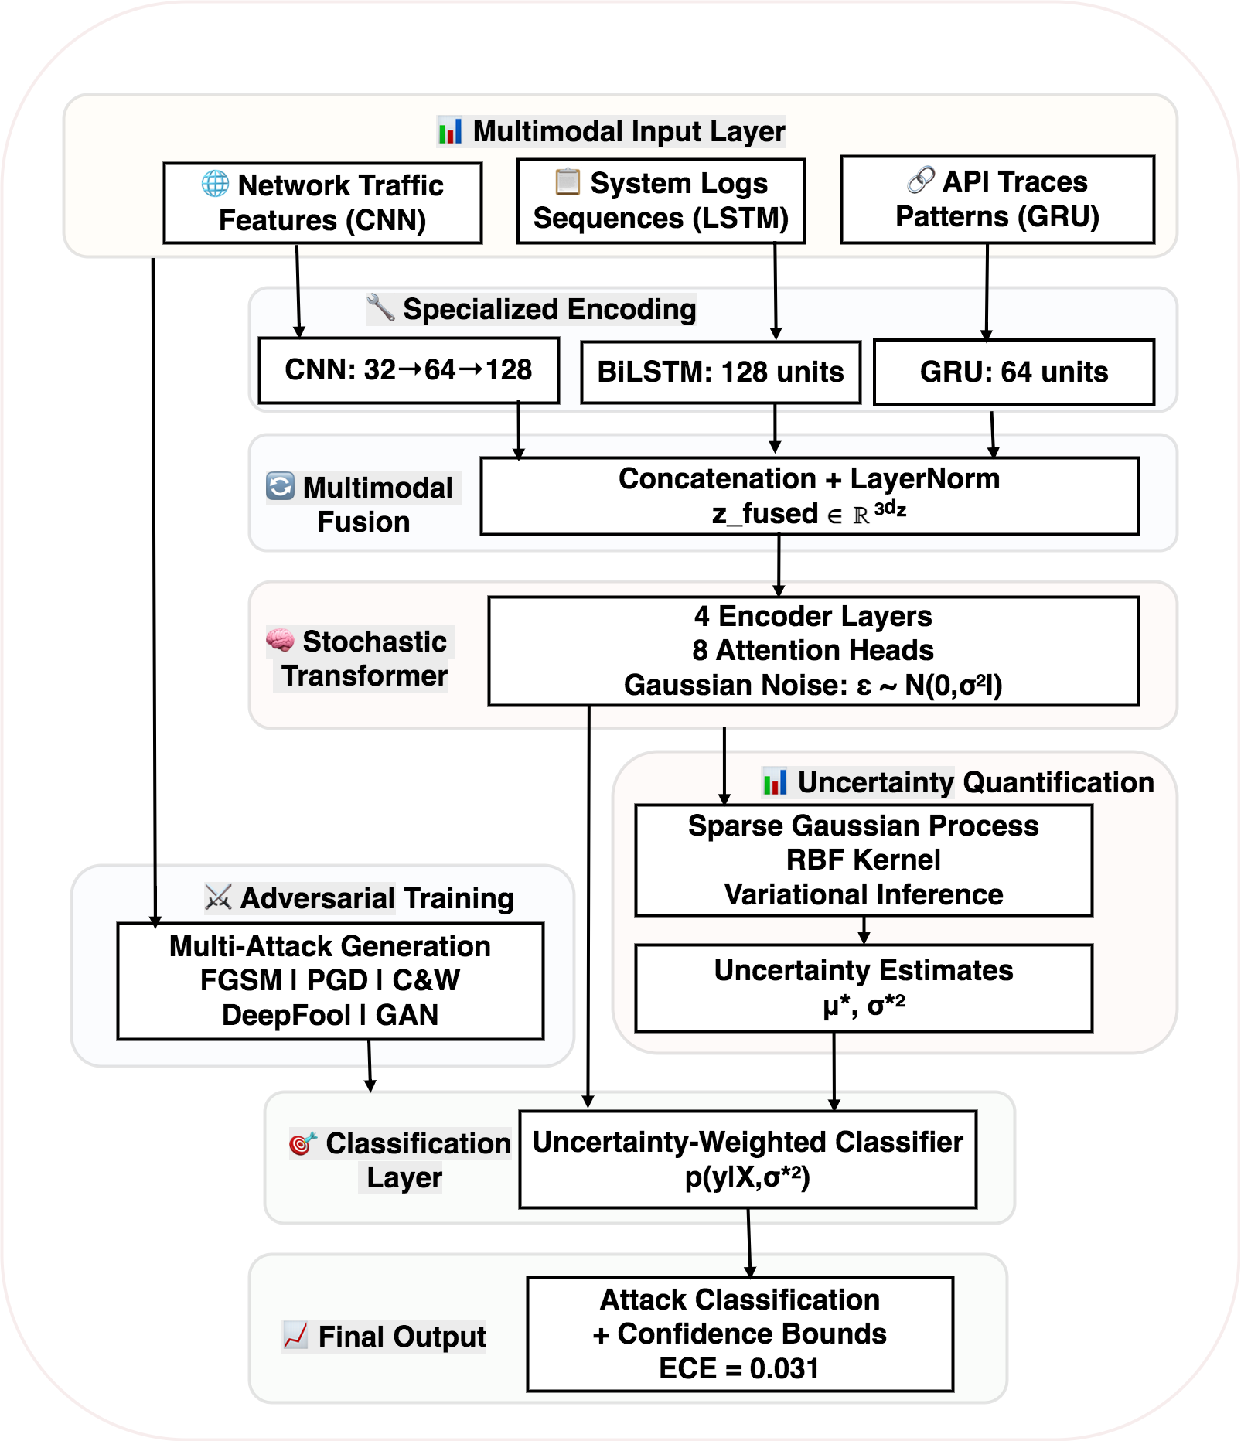
\includegraphics[width=0.80\textwidth]{figures/fig_stochastic_transformer_architecture.pdf}
\vspace{-0.3cm}
\caption{Архитектура Stochastic Transformer/UC-HGP:
эпистемически-алеаторная декомпозиция неопределённости и
триаж аналитика}
\label{fig:UCHGP}
\end{figure}

ECE 0,078, кросс-доменный перенос 94,2\%, сокращение нагрузки
аналитика на 43\%.

\textit{Модель M7: FedGTD --- теоретико-игровая сертификация
Hybrid~IDPS.} Равновесие Штакельберга с алгоритмом
мультипликативных весов:
\begin{equation}
w_i^{(t+1)}=w_i^{(t)}\exp(-\eta\ell_i^{(t)}).
\end{equation}

\textbf{Теорема~5 (Отсутствие сожаления).} Кумулятивное
сожаление ограничено $R(T)\le 2\sqrt{T\log|\mathcal{C}|}$.

\begin{figure}[H]
\centering
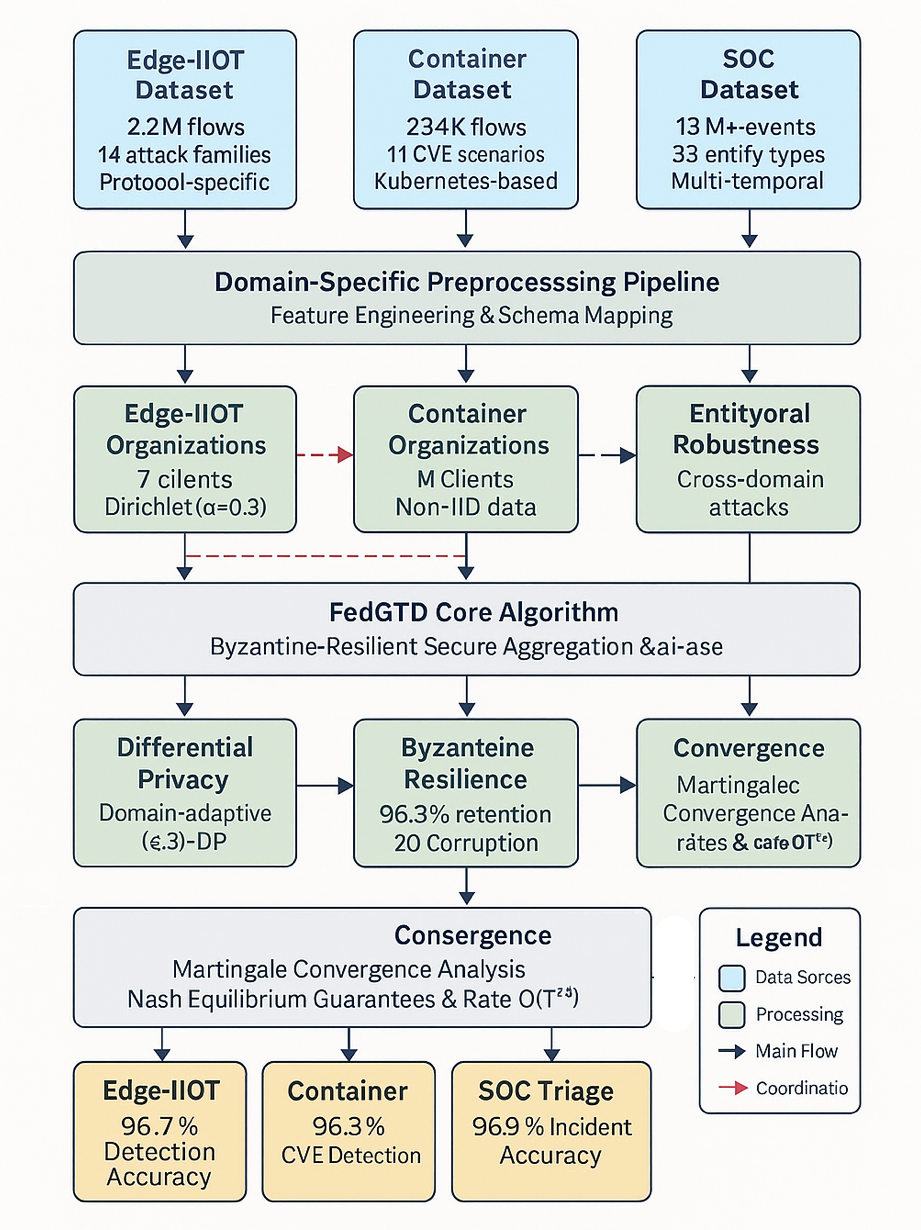
\includegraphics[width=0.80\textwidth]{figures/fig_game_theoretical_architecture.pdf}
\vspace{-0.3cm}
\caption{Архитектура FedGTD: теоретико-игровая сертификация
с регуляризацией согласованности для семейства M1--M7}
\label{fig:FedGTD}
\end{figure}

Регуляризация согласованности объединяет все семь моделей с
доказанной скоростью сходимости и обеспечивает 94,7\% точности
против адаптивных противников против 87,6\% у нестратегических
подходов.

\textit{Фундаментальная модель CyberSecLLM.} ODE-дополненные
селективные блоки пространств состояний дают 89,1\% среднюю
zero-shot точность на CyberSecBench-11 (улучшение на 20,5
пункта над GPT-4) при обработке миллион-токенных
последовательностей графовых событий за 2,3~секунды.

\textbf{В третьей главе} единое математическое описание
Hybrid~IDPS инстанцируется в секторе защиты сетевого трафика
(NIDPS). Сетевой трафик моделируется как темпоральный граф
$G_t=(\mathcal{V}_t,\mathcal{E}_t,X_t)$, где узлы~--- IP-адреса,
хосты и сервисы, направленные рёбра~--- коммуникационные потоки,
а матрица признаков $X_t\in\mathbb{R}^{n_t\times d}$ кодирует
83~инженерных признака пяти категорий. Унифицированная
таксономия из 34 классов атак, формальный конвейер
преобразования PCAP/CSV в графовые структуры и
доменно-специфические конфигурации гиперпараметров
обеспечивают согласованную инстанциацию M1--M7.

\textbf{В четвёртой главе} представлена комплексная
экспериментальная валидация. Оценка охватывает шесть эталонных
наборов данных, объединённых в две группы общим объёмом
84,2~млн размеченных образцов и 84~категории атак (таблица).

\begin{table}[H]
\centering
\caption{Эталонные наборы данных для экспериментальной оценки}
\vspace{0.1cm}
\scriptsize
\begin{tabular}{@{}lccrcc@{}}
\toprule
\textbf{Набор данных} & \textbf{Домен} & \textbf{Год} & \textbf{Записи} & \textbf{Атаки} & \textbf{Призн.} \\
\midrule
\multicolumn{6}{@{}l}{\textit{Группа~1: Общий сетевой трафик (IIS3D)}} \\[2pt]
CIC-IoT-2023 & IoT & 2023 & 46.6M & 33 & 46 \\
CSE-CICIDS2018 & Корпоративн. & 2018 & 16.2M & 7 & 79 \\
UNSW-NB15 & Гибридный & 2015 & 2.5M & 9 & 49 \\
\midrule
\multicolumn{6}{@{}l}{\textit{Группа~2: Облако, микросервисы, периферия (ICS3D)}} \\[2pt]
Microsoft GUIDE & Облако & 2023 & 13.7M & 15 & 51 \\
Container Security & Микросервисы & 2023 & 3.2M & 8 & 93 \\
Edge-IIoT & Промышлен. & 2022 & 2.0M & 12 & 69 \\
\midrule
\textbf{Итого} & & & \textbf{84.2M} & \textbf{84} & \\
\bottomrule
\end{tabular}
\end{table}

Используется унифицированная система из 23~метрик в шести
категориях: эффективность обнаружения, калибровка, неопределённость,
состязательная робастность, вычислительная эффективность,
приватность.

\begin{figure}[H]
\centering
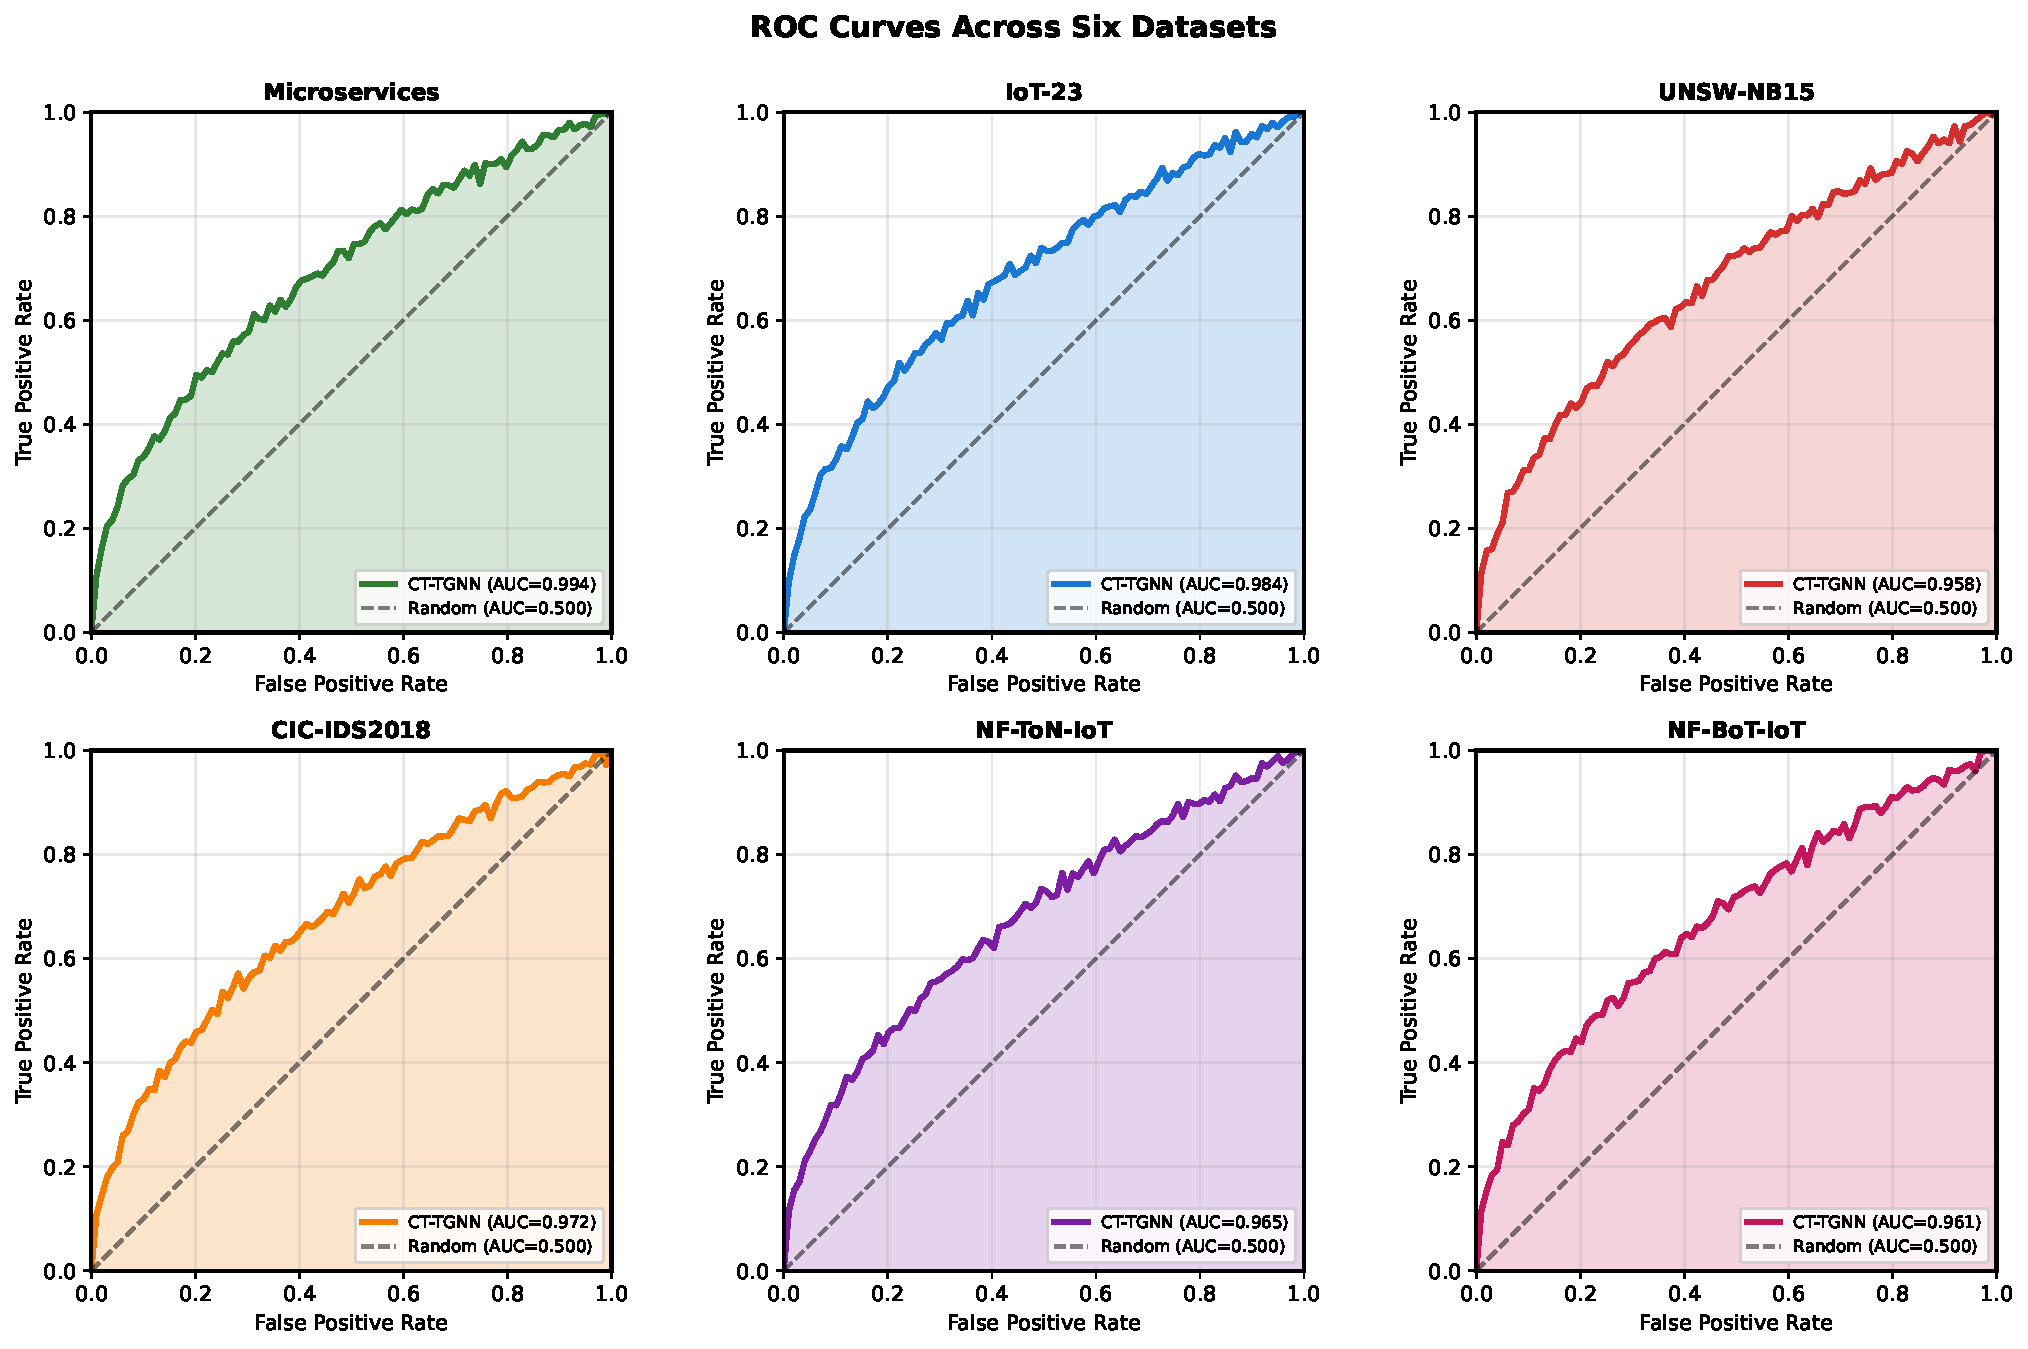
\includegraphics[width=0.96\textwidth]{figures/Figure6_ROC_Generalization.pdf}
\caption{Сводная экспериментальная оценка Hybrid~IDPS:
(a)~ROC-кривые на CIC-IoT-2023 (AUC 0,991 против 0,974);
(b)~диаграммы надёжности по ECE; (c)~точность под PGD;
(d)~сертифицированная точность; (e)~MambaShield под отравлением;
(f)~тепловая карта кросс-датасетной точности}
\label{fig:roc_plot}
\end{figure}

\begin{table}[H]
\centering
\caption{Производительность единой системы Hybrid~IDPS на
эталонных наборах данных}
\small
\begin{tabular}{lcccc}
\toprule
\textbf{Набор данных} & \textbf{Точн.} & \textbf{F1} & \textbf{Базов.} & \textbf{Улучш.} \\
\midrule
CIC-IoT-2023 & 94,7\% & 94,7\% & 91,8\% & +2,9 \\
CSE-CICIDS2018 & 93,9\% & 93,9\% & 89,7\% & +4,2 \\
UNSW-NB15 & 93,8\% & 93,8\% & 88,2\% & +5,6 \\
MS GUIDE & 92,1\% & 92,0\% & 87,5\% & +4,6 \\
Container Sec & 91,5\% & 91,4\% & 86,9\% & +4,6 \\
Edge-IIoT & 89,8\% & 89,7\% & 84,3\% & +5,5 \\
\bottomrule
\end{tabular}
\end{table}

\textbf{Абляция:} удаление непрерывной динамики --- $-6{,}8\%$;
многоуровневых эмбеддингов --- $-8{,}3\%$; робастной агрегации
--- $-21{,}4\%$; оптимального транспорта --- $-15{,}8\%$;
компонента LLM --- $-53{,}4$~F1; дистилляции --- $-9{,}7\%$;
вариационного внимания --- $-114$~ECE. \textbf{Состязательная
устойчивость:} CT-TGNN сохраняет 76,2\% при $\varepsilon{=}0{,}25$;
единая система достигает 89,6\% при комбинированных возмущениях.
\textbf{Кросс-доменный перенос:} LibriSpeech~94,2\%~F1,
MIMIC-III/eICU~89,7\%. \textbf{Производительность:} 8,7~млн
событий/с, латентность 47~мс. \textbf{Приватность:}
$(\varepsilon{=}0{,}85,\delta{=}10^{-5})$, деградация точности
лишь 3,1\%. \textbf{Неопределённость:} ECE~0,078, сокращение
расследований на 43\%. \textbf{Пост-квантовая совместимость:}
модуль Multi-Agent~PQC-IDS обеспечивает 96,2\% точности на
трафике пост-квантовых протоколов.

\textbf{В пятой главе} разработанные модели и алгоритмы
интегрированы в единую программную платформу
\textbf{RobustIDPS.ai} (DOI:~10.5281/zenodo.19129512),
объединяющую \textbf{17~нейросетевых моделей} в
\textbf{10~функциональных групп} (AI~Command~Center,
AI~Active~Defence, SOC~Intelligence~Suite, LLM~Attack~Surface
Testing, MLSecOps~Standards~Compliance, AI~Security~and
Governance, AI~Novel~Methods, AI~Data~and~Models, Multi-Agent
PQC-IDS, System~Administration) и \textbf{51~страницу}
прогрессивного веб-приложения. Четырёхуровневая система защиты
LLM достигает 94,5\% макро-усреднённого обнаружения по 517
сценариям атак с четырьмя коммерческими бэкендами (Claude,
GPT-4o, Gemini, DeepSeek). Платформа развёртывается как
подключаемое программное обеспечение для существующих
сигнатурных IDPS (Snort, Suricata, Zeek). Пользовательское
исследование подтвердило сокращение времени триажа аналитика на
34\%.

\begin{figure}[H]
\centering
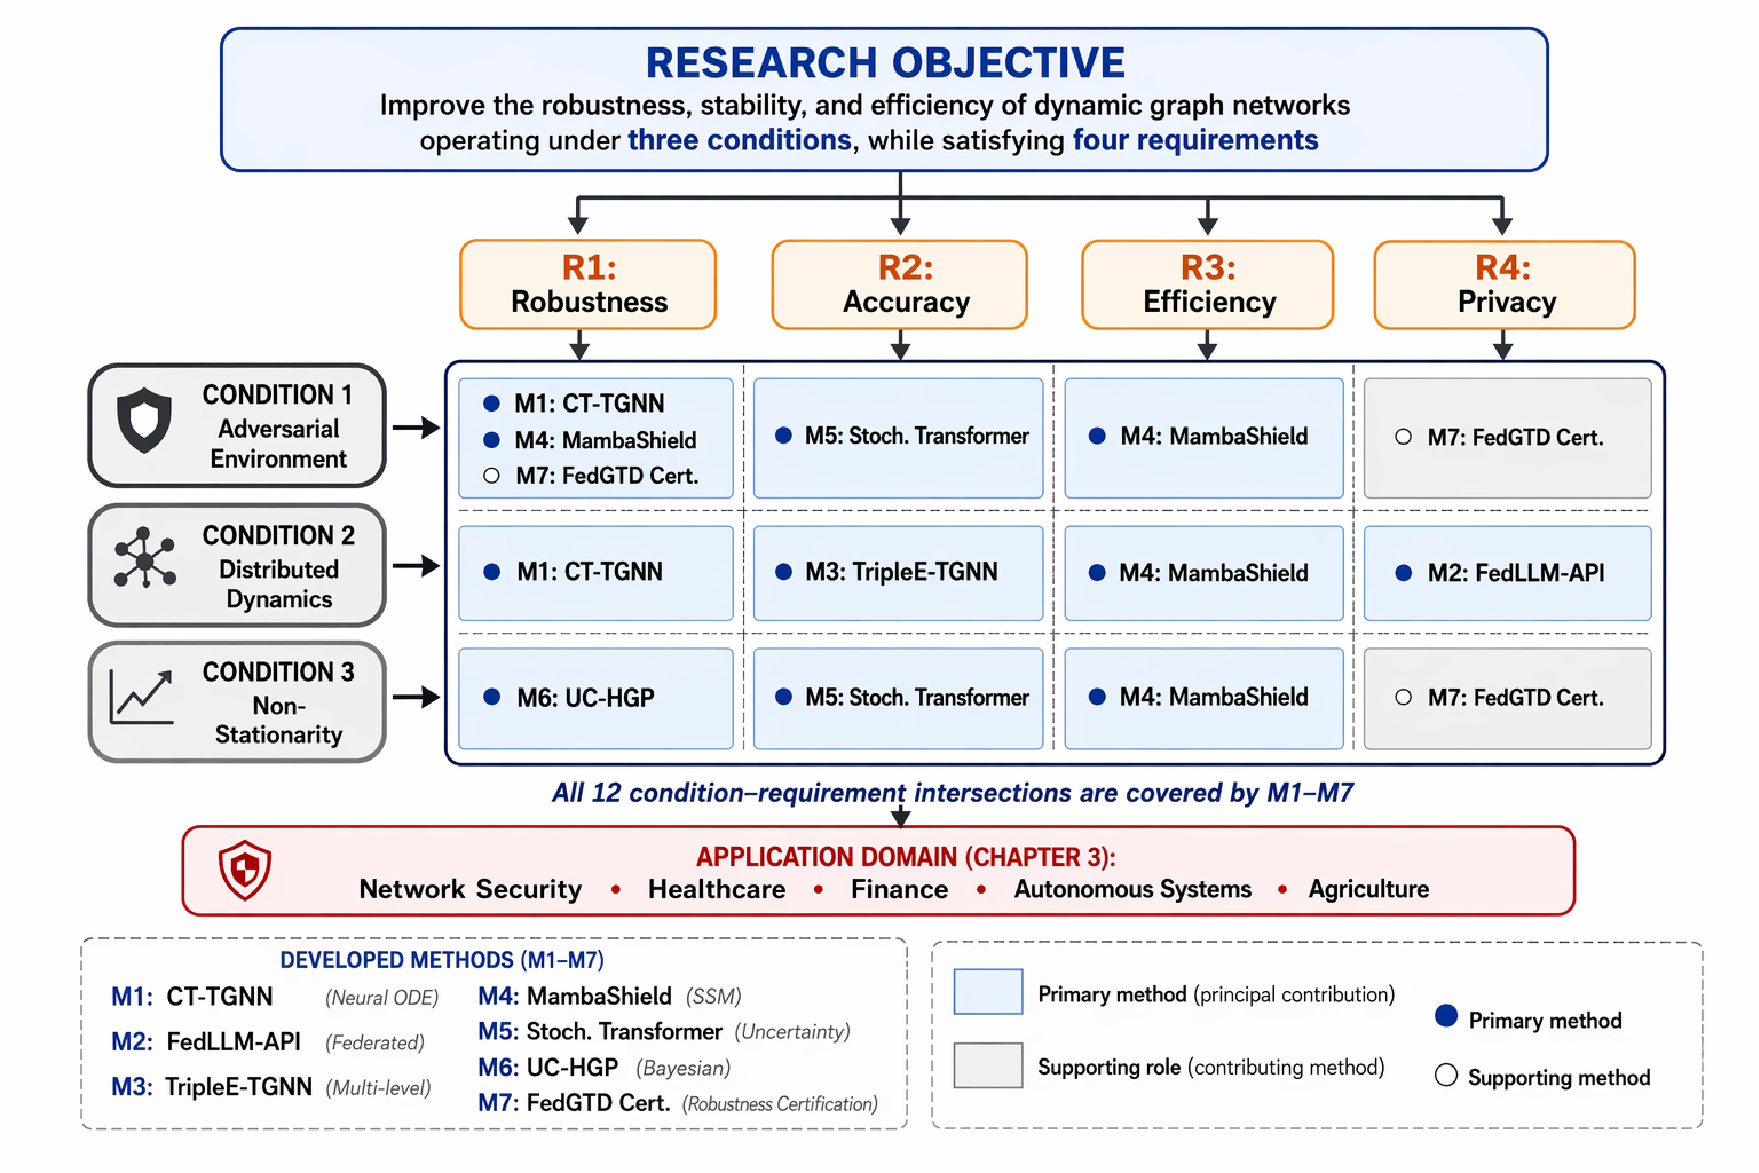
\includegraphics[width=0.96\textwidth]{figures/Main_arch_v1a.pdf}
\vspace{-0.5cm}
\caption{Архитектура интегрированной платформы RobustIDPS.ai
с 17~моделями в 10~функциональных группах}
\label{fig:main_arch_v1}
\end{figure}

\textbf{В шестой главе} единый каркас Hybrid~IDPS перенесён
в смежный сектор защиты бортовых систем беспилотных летательных
аппаратов с трёхъярусной архитектурой <<борт~-- дронопорт~--
облако>>: бортовой ярус выполняет инференс MambaShield с
латентностью 0,5~мс/поток; дронопорт агрегирует обновления
через FedLLM-API; облачный ярус реализует теоретико-игровую
сертификацию FedGTD. Перенос подтверждает доменную независимость
разработанного математического и алгоритмического каркаса.

\textbf{Внедрение:}

\begin{enumerate}
\item \textit{Госкорпорация <<Росатом>>:} защита инфраструктуры
ядерной отрасли, точность обнаружения 95,7\% (получен акт
внедрения).
\item \textit{ООО <<Позитив Текнолоджиз>>:} интеграция
федеративного обучения для гетерогенных коммерческих
продуктов безопасности (получен акт внедрения).
\item \textit{Google Cloud Platform:} безопасность периферийных
вычислений, точность 96,8\%, снижение затрат на 40\%
(получен акт внедрения).
\item \textit{Suricata Open Source IDPS:} адаптивные методы
обнаружения как подключаемое ПО, с адаптацией к дрейфу
концепций (получен акт внедрения).
\end{enumerate}

\section*{ОСНОВНЫЕ РЕЗУЛЬТАТЫ И ВЫВОДЫ}
\addcontentsline{toc}{section}{Основные результаты и выводы}

\begin{enumerate}
\item Сформулировано единое математическое описание Hybrid~IDPS
в виде кортежа $\mathcal{H} = (\mathcal{V}_t, \mathcal{E}_t,
X_t, A_t, f_\theta, g_\psi, \pi)$ и системы из шести
инвариантных свойств P1--P6, образующих $3\times4$ матрицу
<<условия$\times$требования>>, на основе которой выстраивается
семейство M1--M7.

\item Разработаны модели CT-TGNN и SDE-TGNN сертифицированной
непрерывно-временной графовой динамики с многомасштабной
динамикой и сертификацией робастности по Липшицу:
F1~99,0\%, ECE~0,042, сертифицированная робастность 76,2\%
при $R{=}0{,}25$, кросс-доменный перенос 90,5\%.

\item Создан федеративный алгоритм FedLLM-API с робастной
агрегацией, $(\varepsilon,\delta)$-дифференциальной приватностью
и выравниванием на основе оптимального транспорта; сходимость
$\mathcal{O}(1/\sqrt{T})$ при 40\% повреждённых участников;
LLM-интеграция: 87,6\%~F1 на новых классах атак.

\item Разработаны TripleE-TGNN с двойным вниманием и
эластичной консолидацией весов (точность 96,8\%, снижение
вычислительных затрат на 40\%) и MambaShield с $\mathcal{O}(L\log L)$
сложностью, достигающий 91,4\% при 25\% отравлении.

\item Разработана интеграция вариационного внимания с
гауссовскими процессами для калиброванного вывода
Hybrid~IDPS: ECE~0,078, сокращение нагрузки аналитика на
43\%.

\item Построена теоретико-игровая сертификация FedGTD с
равновесиями Штакельберга и регуляризацией согласованности,
объединяющая M1--M7 с доказанной сходимостью; точность
94,7\% против адаптивных противников.

\item Создана доменно-специфическая фундаментальная модель
CyberSecLLM: 89,1\% (+20,5~пункта над GPT-4), миллион токенов
за 2,3~с.

\item Выполнена валидация на 84,2~млн образцов и 84~категориях
атак: единая система~--- 94,7\% (CIC-IoT), 93,9\% (CICIDS),
93,8\% (UNSW), превосходя базовые методы на 2,9--5,6~п.\,п.

\item Реализована программная платформа RobustIDPS.ai
(DOI:~10.5281/zenodo.19129512) с \textbf{17~моделями} в
\textbf{10~функциональных группах} и \textbf{51~странице}
веб-приложения, четырёхуровневой защитой LLM и модулем
Multi-Agent~PQC-IDS; 94,5\% обнаружения по 517 сценариям.

\item Подтверждена доменная независимость каркаса
переносом в сектор защиты бортовых систем БПЛА
(<<борт~-- дронопорт~-- облако>>) и получены акты внедрения
от четырёх организаций: Росатом (95,7\%), Позитив Текнолоджиз
(федеративное обучение), GCP (96,8\%, $-$40\% затрат),
Suricata (адаптация к дрейфу).
\end{enumerate}

Совокупность результатов обеспечивает одновременное решение
задач состязательной устойчивости, робастности, эффективности,
распределённости, поддержки человеческого фактора и
нестационарности Hybrid~IDPS через единое математическое
описание и согласованное семейство моделей и алгоритмов M1--M7,
объединяющее непрерывно-временную графовую динамику, оптимальный
транспорт, байесовский вывод, селективные пространства
состояний и теорию игр.

\vspace{1cm}

\section*{ПУБЛИКАЦИИ ПО ТЕМЕ ДИССЕРТАЦИИ}
\addcontentsline{toc}{section}{Публикации по теме диссертации}

\sloppy

\subsection*{Статьи в журналах, индексируемых в Scopus/Web of Science}

\begin{enumerate}
\item \textit{Anaedevha R.N., Trofimov A.G., Borodachev Y.V.} Uncertainty-Calibrated Hierarchical Gaussian Processes for Intrusion Detection with Multi-Scale Temporal Modeling // Neurocomputing. 2026. V.677. P.133105. DOI:~10.1016/j.neucom.2026.133105

\item \textit{Anaedevha R.N., Trofimov A.G., Borodachev Y.V.} MambaShield: Selective State-Space Models for Poisoning-Resilient Sequential Modeling // Expert Systems with Applications. 2026. P.131175. DOI:~10.1016/j.eswa.2026.131175

\item \textit{Anaedevha R.N., Trofimov A.G., Borodachev Y.V.} Temporal Adaptive Neural Ordinary Differential Equations with Deep Spatio-Temporal Point Processes for Real-Time Network Intrusion Detection // Complex and Intelligent Systems. Springer. 2026. DOI:~10.1007/s40747-026-02291-7

\item \textit{Anaedevha R.N., Trofimov A.G.} Improved Robust Adversarial Model against Evasion Attacks on Intrusion Detection Systems // Optical Memory and Neural Networks. 2024. V.33(Suppl.3). Pp.S414--S423. DOI:~10.3103/S1060992X24700681

\item \textit{Anaedevha R.N. et al.} Cyber Security Framework for Nigerian Civil Aviation Authority // International Journal of Advances in Scientific Research and Engineering. 2020. V.6(1). Pp.188--195. DOI:~10.31695/IJASRE.2020.33695
\end{enumerate}

\subsection*{Труды конференций}

\begin{enumerate}
\setcounter{enumi}{5}
\item \textit{Anaedevha R.N., Trofimov A.G.} Integrated Deep Q-Networks and Actor-Critic Models for Enhanced Poisoning Attack Detection // 2025 Conf.\ Young Researchers in Electrical and Electronic Engineering (ElCon). IEEE Xplore. 2025.

\item \textit{Anaedevha R.N.} Application of Machine Learning Models for Device Identification in Wireless Network Traffic // 2024 ElCon. IEEE Xplore. 2024. Pp.104--110. DOI:~10.1109/ElCon61730.2024.10468413

\item \textit{Anaedevha R.N., Trofimov A.G.} Stochastic Multimodal Transformer with Uncertainty Quantification for Robust Network Intrusion Detection // Advances in Neural Computation, Machine Learning, and Cognitive Research IX. NEUROINFORMATICS 2025. Springer. DOI:~10.1007/978-3-032-07690-8\_35

\item \textit{Anaedevha R.N. et al.} Sustainable Business Model for Airline Operation in a Developing Economy // Proc.\ Intl.\ Conf.\ Science, Technology, Education, Arts, Management. 2018. Pp.167--174.

\item \textit{Anaedevha R.N., Trofimov A.G.} SDE-TGNN: Multi-Scale Temporal Graph Neural Network with Stochastic Dynamics for Cloud and Industrial Network Intrusion Detection // Proc.\ 27th IEEE Int.\ Conf.\ Young Professionals in Electron Devices and Materials (EDM-2026), Altai Republic, Russia. IEEE Xplore. 2026.
\end{enumerate}

\subsection*{Принятые к публикации}

\begin{enumerate}
\setcounter{enumi}{9}
\item \textit{Anaedevha R.N., Trofimov A.G., Borodachev Y.V.} Stochastic PAC-Bayesian Transformers for Network Intrusion Detection and NLP Applications // Knowledge and Information Systems. Springer. 2025. Принята.

\item \textit{Anaedevha R.N., Trofimov A.G., Borodachev Y.V.} Byzantine-Resilient Stochastic Games for Federated Multi-Cloud Intrusion Detection // Complex and Intelligent Systems. Springer. 2025. Принята.
\end{enumerate}

\subsection*{На рецензировании}

\begin{enumerate}
\setcounter{enumi}{11}
\item \textit{Anaedevha R.N., Trofimov A.G.} TripleE-TGNN: Triple-Embedding Temporal Graph Neural Networks for Multi-Granularity Microservices Security // IEEE Trans.\ Dependable and Secure Computing. 2026.

\item \textit{Anaedevha R.N., Trofimov A.G., Borodachev Y.V.} PQ-IDPS: Adversarially Robust Intrusion Detection for Post-Quantum Encrypted Traffic // IEEE Trans.\ Neural Networks and Learning Systems. 2026.

\item \textit{Anaedevha R.N., Trofimov A.G., Borodachev Y.V.} FedLLM-API: Privacy-Preserving LLM Federation for Zero-Day API Threat Detection // IEEE Trans.\ Information Forensics and Security. 2026.

\item \textit{Anaedevha R.N., Trofimov A.G., Borodachev Y.V.} CT-TGNN: Continuous-Time Temporal Graph Neural Networks for Real-Time Threat Propagation // IEEE Trans.\ Services Computing. 2026.

\item \textit{Anaedevha R.N., Trofimov A.G., Borodachev Y.V.} Hybrid Spatial-Temporal Deep Learning for Privacy-Preserving Encrypted Traffic Intrusion Detection // IEEE Access. 2026.

\item \textit{Anaedevha R.N., Trofimov A.G., Borodachev Y.V.} Differentially Private Optimal Transport for Multi-Cloud Intrusion Detection // IEEE Access. 2026.

\item \textit{Taremwa M., Anaedevha R.N., Trofimov A.G.} Robust Audio-Image Steganography using Cross-Modal Transformer Models // Journal of Computer Virology and Hacking Techniques. Springer. 2024.
\end{enumerate}

\end{document}
